\chapter{Hardware Implementation}

\section{Hardware choices}
With the specification and design phase of the 16-bit breadboard computer now complete,
the next step towards having a woking and functional computer was to make some judicious
hardware choices. First up, the breadboards had to be chosen.

\subsection{Breadboard selection}
Following Ben Eater's advice \cite{eater2020breaboards}, the first choice of breadboards
was the \emph{BB830} from \emph{BusBoard Technologies}, retailed by \emph{Mouser}
\cite{mouser2020breadboards}. Unfortunately, due to limited stock at the time, only 10 such
breadboard could be aquired. Because of this, a compromise had to be met. The rest of the boards
bought were cheaper BB830 clones retailed by \emph{Farnell} \cite{farnell2020breadboards}.
The operating principle of a breadboard is that each vertical column of 5 pin is connected,
together, as well as the horizontal top and bottom two rows which provide power and ground.
The way breadboards provide resilient connections without using solder is by having small metal
clamps inside the pin holes which, when pried apart by an inserted pin, will rub against it
and, as suh, provide high quality contact points. The main issue which could arrise from using
low quality breadboards is the fact that, after only a few pin insertions, the metal clamps
loose their elastical properties and stay pried open, not making contact anymore. Since the plan
is to insert all components once and then leave them in their position, this issue shouldn't
manifest itself.
Besides breadboard choice, how to connect multiple breadboards is also an important question.
The boards are modular, meaning that each board can have its two power deliver strips removed.
By only removing one strip from each board, two breadboards can be connected together and each
board will still have two power strps: one at the top and one at the bottom. The extra power strips
can be connected together and used to build up the common bus at the center of the computer.
Unfortunatley, due to the large size of the computer, it became clear that the strips removed
from breadboards wouldn't be enough to cover the entire length. Fortunatley, \emph{Farnell} stocked
the power strips as separate items, so a few of those were purchased \cite{farnell2020strips}.
Given the number pins on each breadboard and the number of pins on all required chips, the number
of required breadboards could be calculated. This calculation lead to the creation of a simple
schematic which details how each module is organized on breadboards \ref{module_layout}.

\begin{figure}[h]
  \centering
  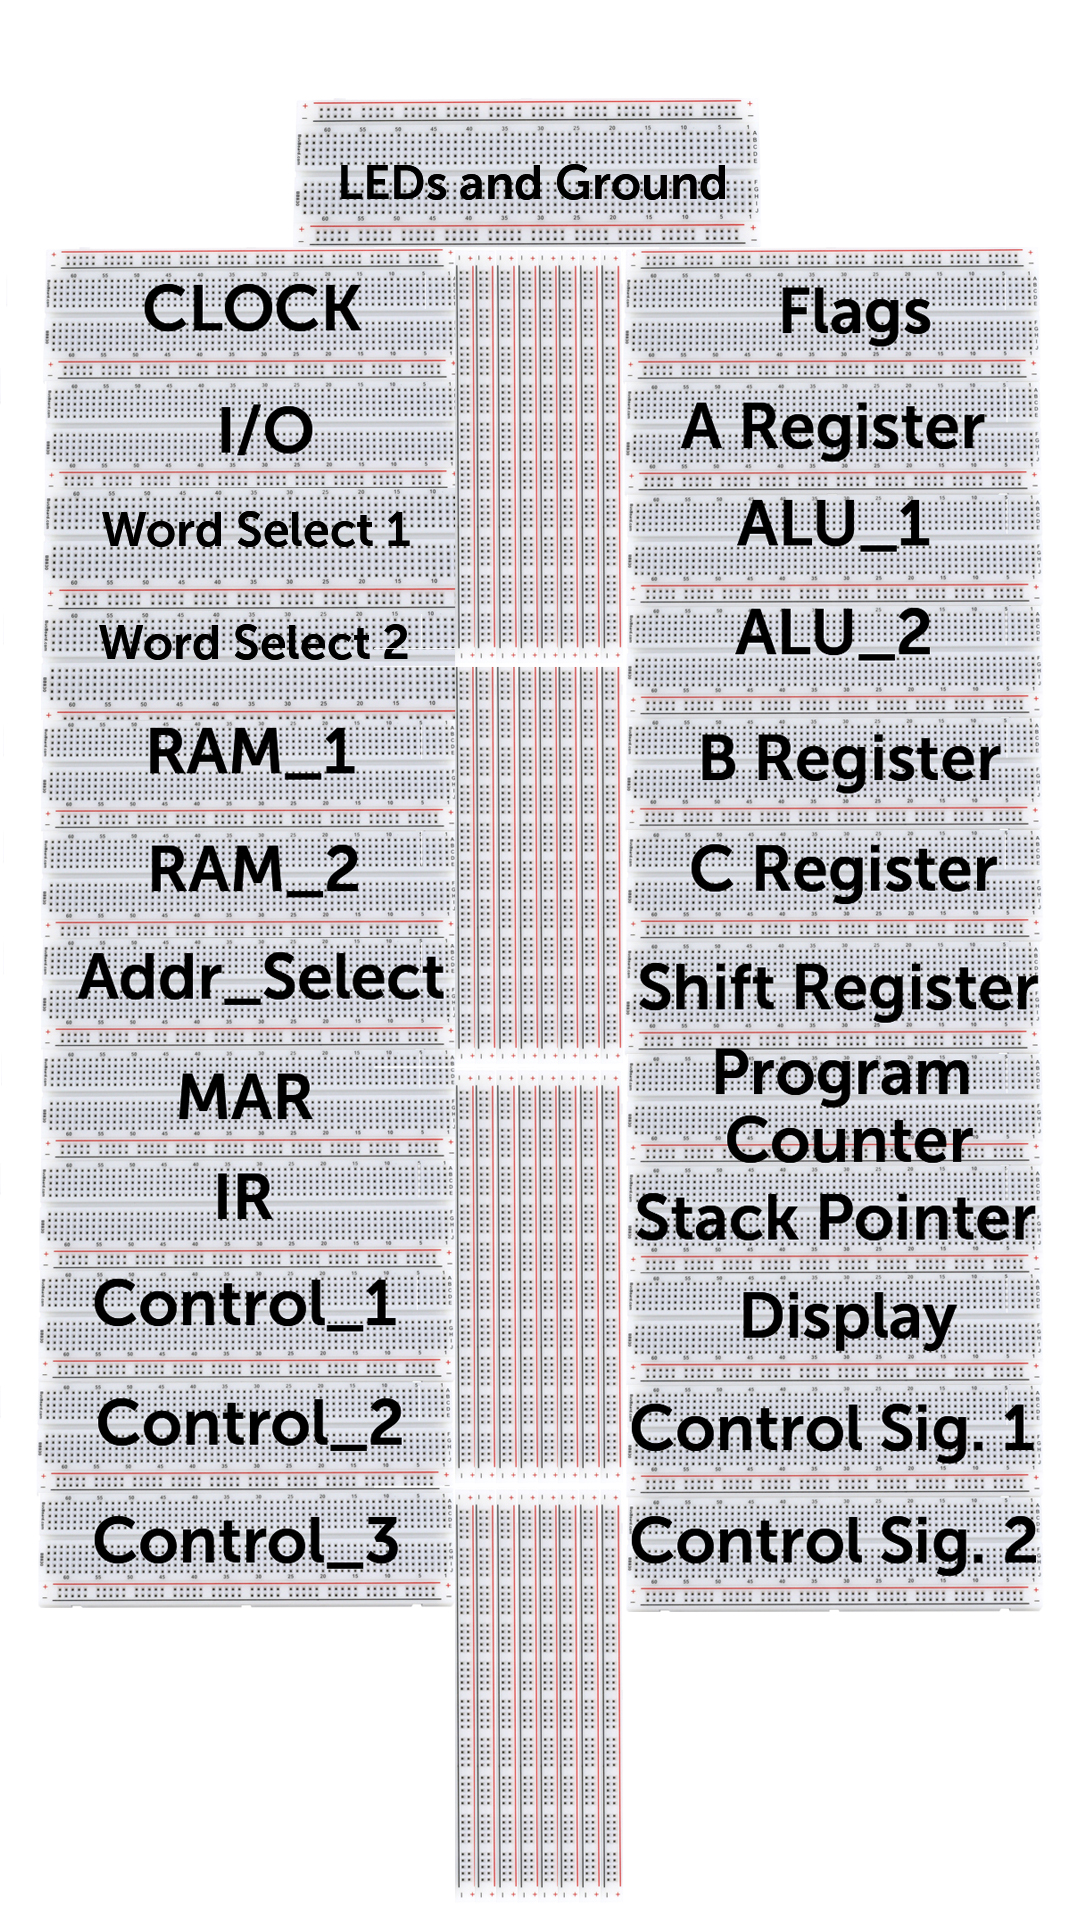
\includegraphics[scale=0.20]{BreadBoardCompLayout}
  \caption{Module Layout onto BB830 breadboards}
  \label{module_layout}
\end{figure}
\pagebreak

\subsection{Wire choice}
The choice of wires was mostly based on the breadboards. According to the specification provide
by \emph{BusBoard} \cite{multicomp2020breadboards}, the BB830 can use wires of thickness ranging
between 29AWG and 20AWG. Multiple 10 meter spools of PVC-insulated multi-coloured 22AWG monofilar
copper wires were purchased. The multiple colors were mapped as follows to different functions
in the computer:
\begin{itemize}
  \item Red: Power (+5V/VCC)
  \item Black: Ground (GND)
  \item Purple, Brown and Orange: Internal module connections
  \item Blue: Bus connections
  \item Green: Control signals
  \item Yellow: Clock signal and Arduino Connections
\end{itemize}
Purple, Brown and Orange ran out towards the end of the build phase (Control Logic), so Green,
Yellow and Blue was used.

\subsection{Power Delivery}
One important area which was glossed over during the Specification and Design phase was the power
delivery. While it is convenient to assume easy access to perfect 5V voltage accross all modules,
in practice this is not trivial to achieve. Besides this, there are also current limitations to
take into account.

\subsubsection{Main Power Delivery}
Ben Eater uses in his build a simple 5V USB wall charger usually used for phones, from which he
cut off the microUSB connector and soldered a barrel connector to the 5V and Ground leads
\cite{eater2020power}. This has also been attempted for the 16-bit breadboard computer, but it
quickly became apparent that, given the many more components used in this upgraded and extended
version,  the current draw far exceeded the 1A current limit of the phone charger. As such, a more
robust power solution was required. Since there was no laboratory power supply available, an old
and discarded ATX 450 Watt power supply was used \ref{psu}. This power supply has a current limit
of 35A on the 5V rail, so it should manage to supply the 16-bit breadboard computer with as much
current as needed. To interface the power supply to the computer, an ATX power connector was de-
soldered from an old PC motherboard, and then cable bundles were soldered on to the 5V and Ground
pins of the connector \ref{atx}. Those cables were then inserted into a power strip at the top of
the computer, near the LEDs module \ref{power_strip}. Finally, two pairs of 5V plus Ground cables
were routed from the power strip to each breadboard \ref{power_conn}. This ensured that each
power strip was at a relativley equal resistance from the main power strip, so the voltage across
strips was essentially equal. This also ensured that the breadboards would have enough current
draw available, as each module was connected more or less directly to the PSU. After testing
random voltage samples across all breadboards using a multimeter, the average voltage was found
to be around 4.8 Volts, which is well within the specification of the chips used (the
specification usually states that the chips work in a 4.75 - 5.25 Volts voltage range).

\begin{figure}[ht]
  \centering
  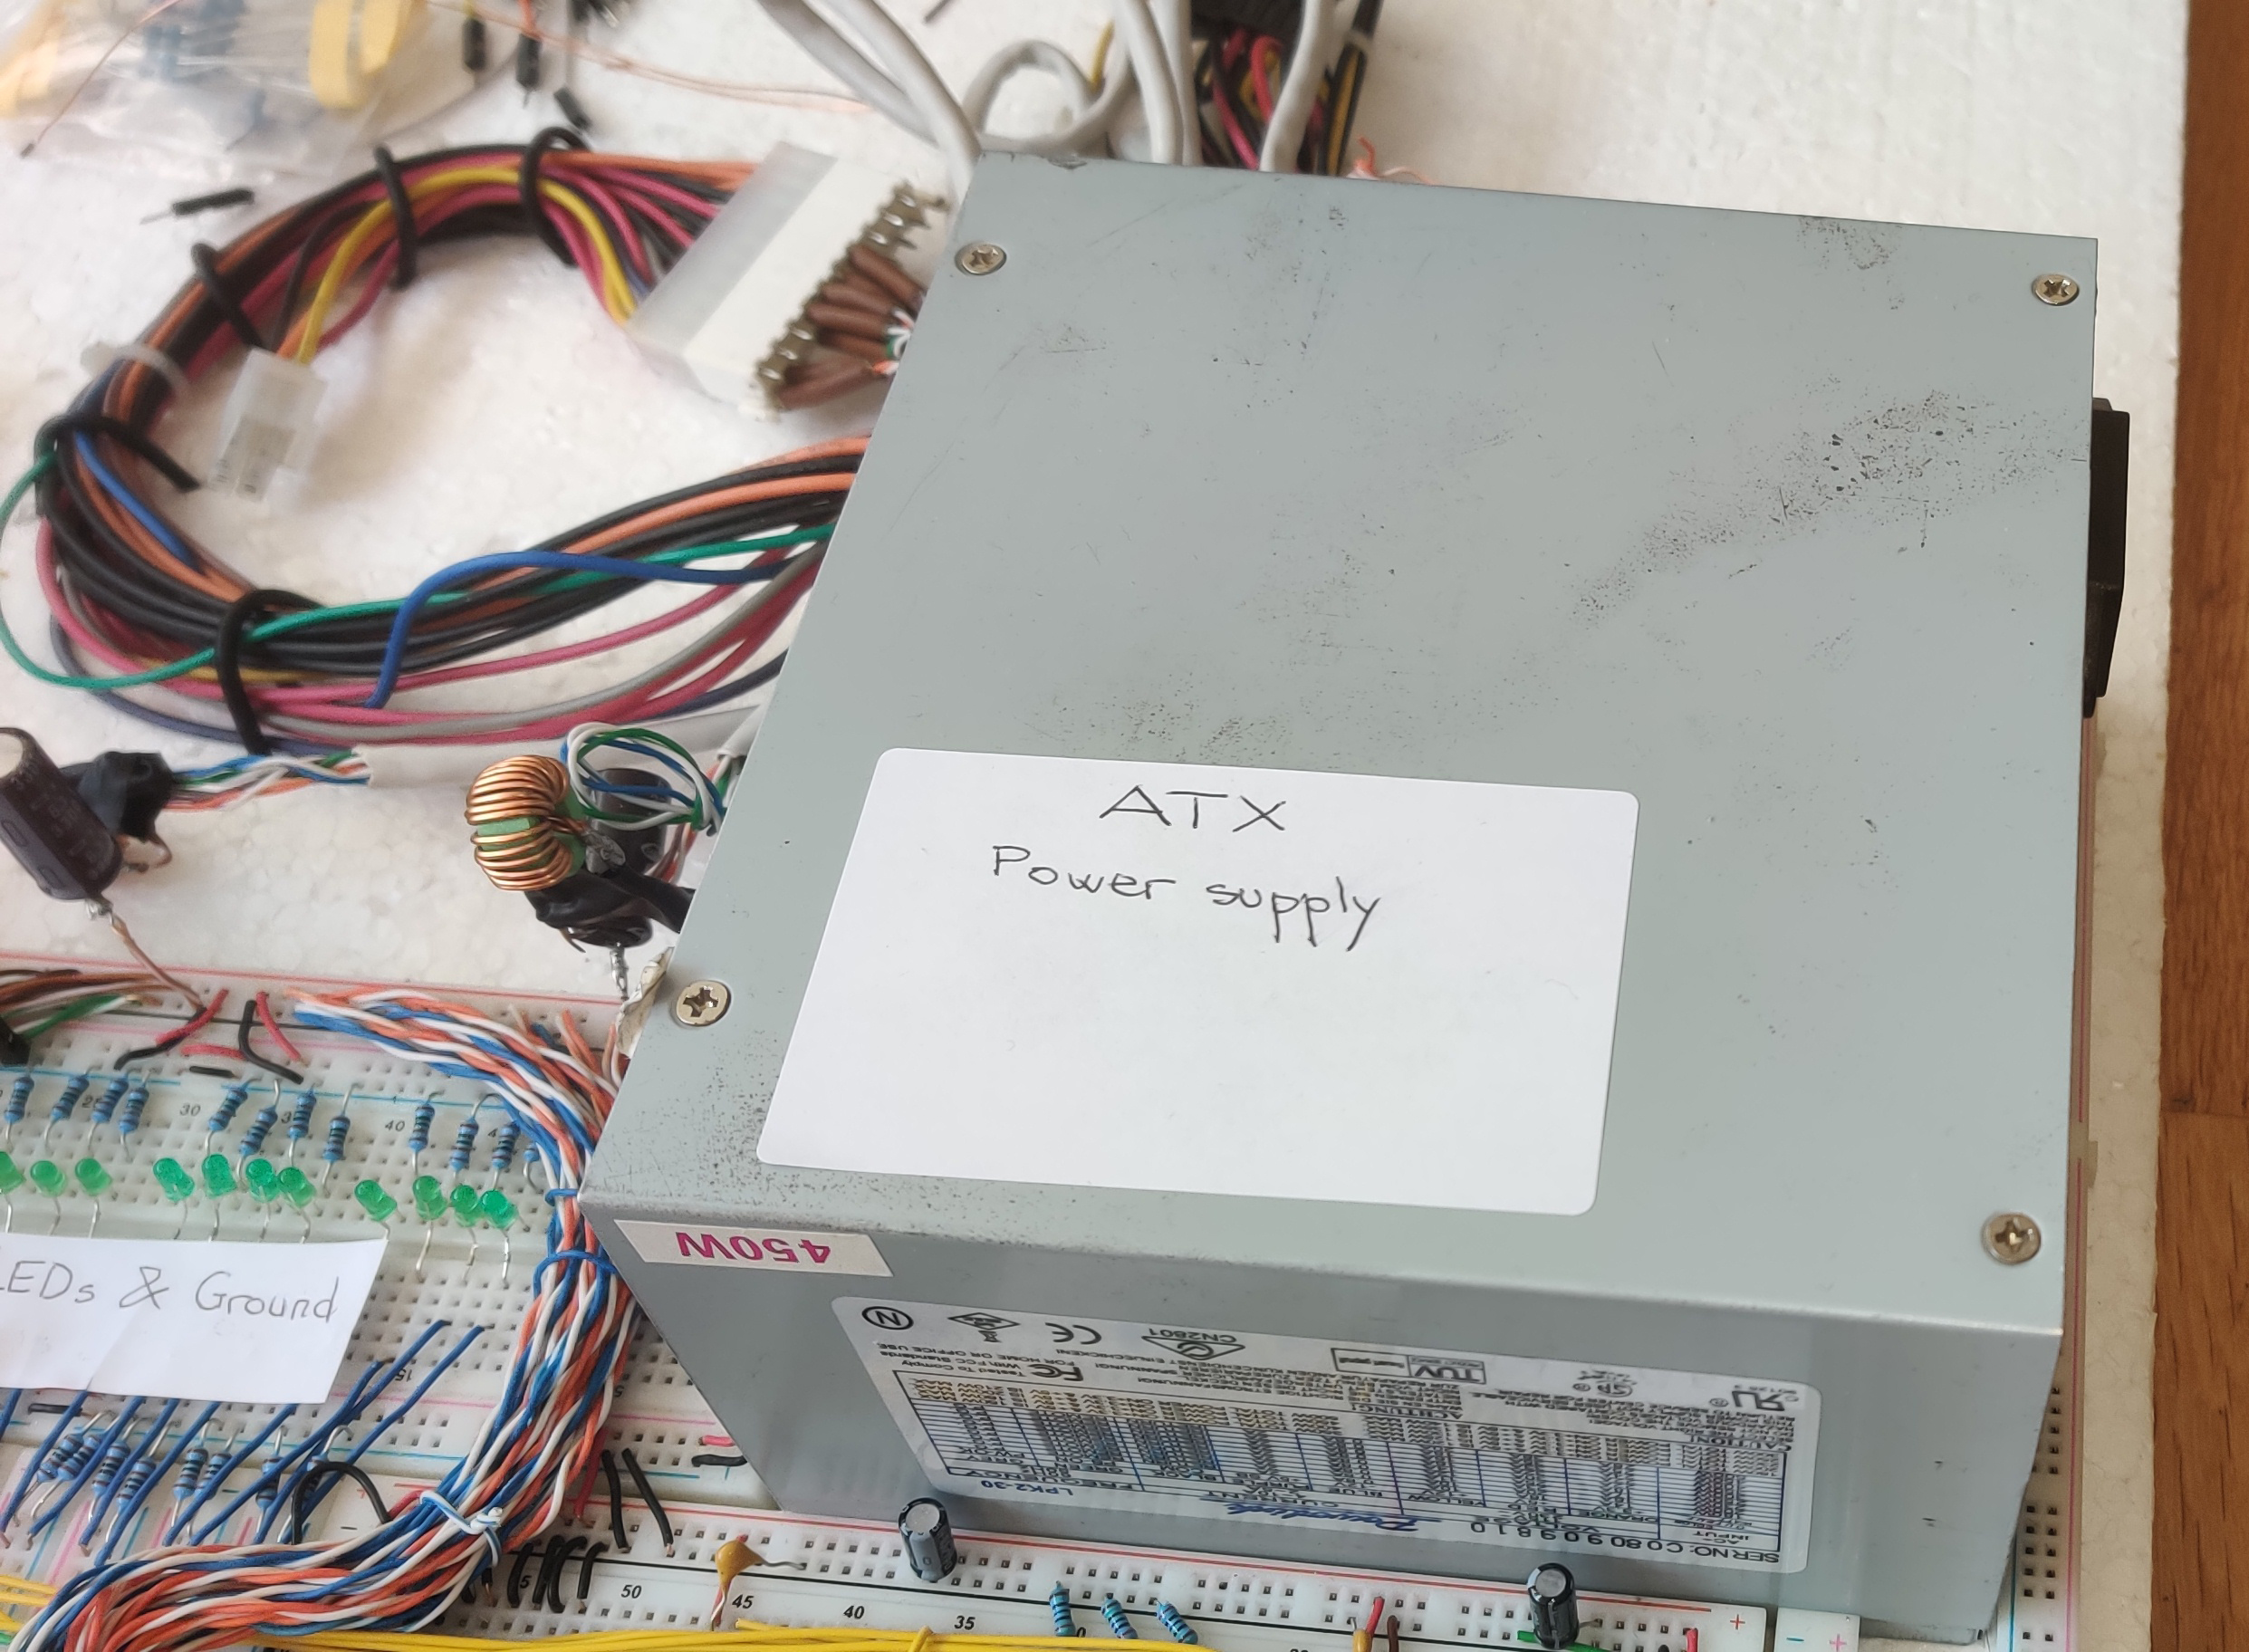
\includegraphics[scale=0.1]{psu}
  \caption{450W ATX Power Supply used to provide 5V power to the breadboard computer }
  \label{psu}
\end{figure}

\begin{figure}[ht]
  \centering
  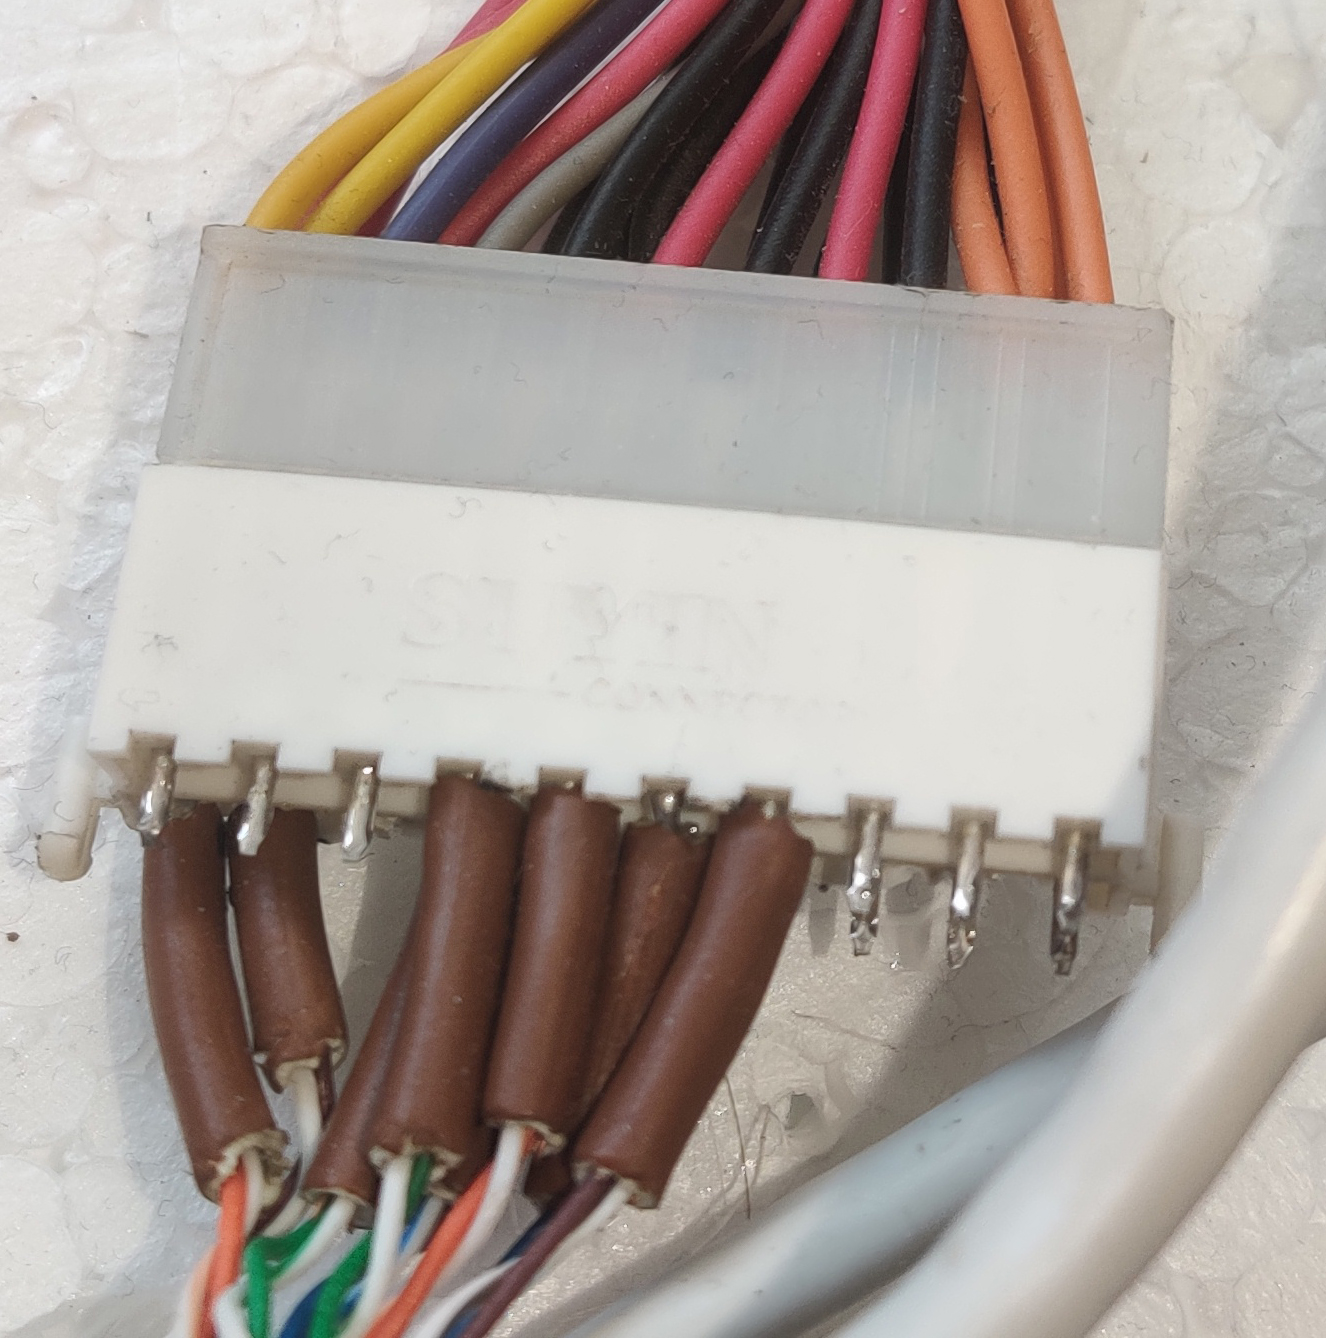
\includegraphics[scale=0.2]{atx}
  \caption{ATX connector salvaged from an old motherboard}
  \label{atx}
\end{figure}

\begin{figure}[ht]
  \centering
  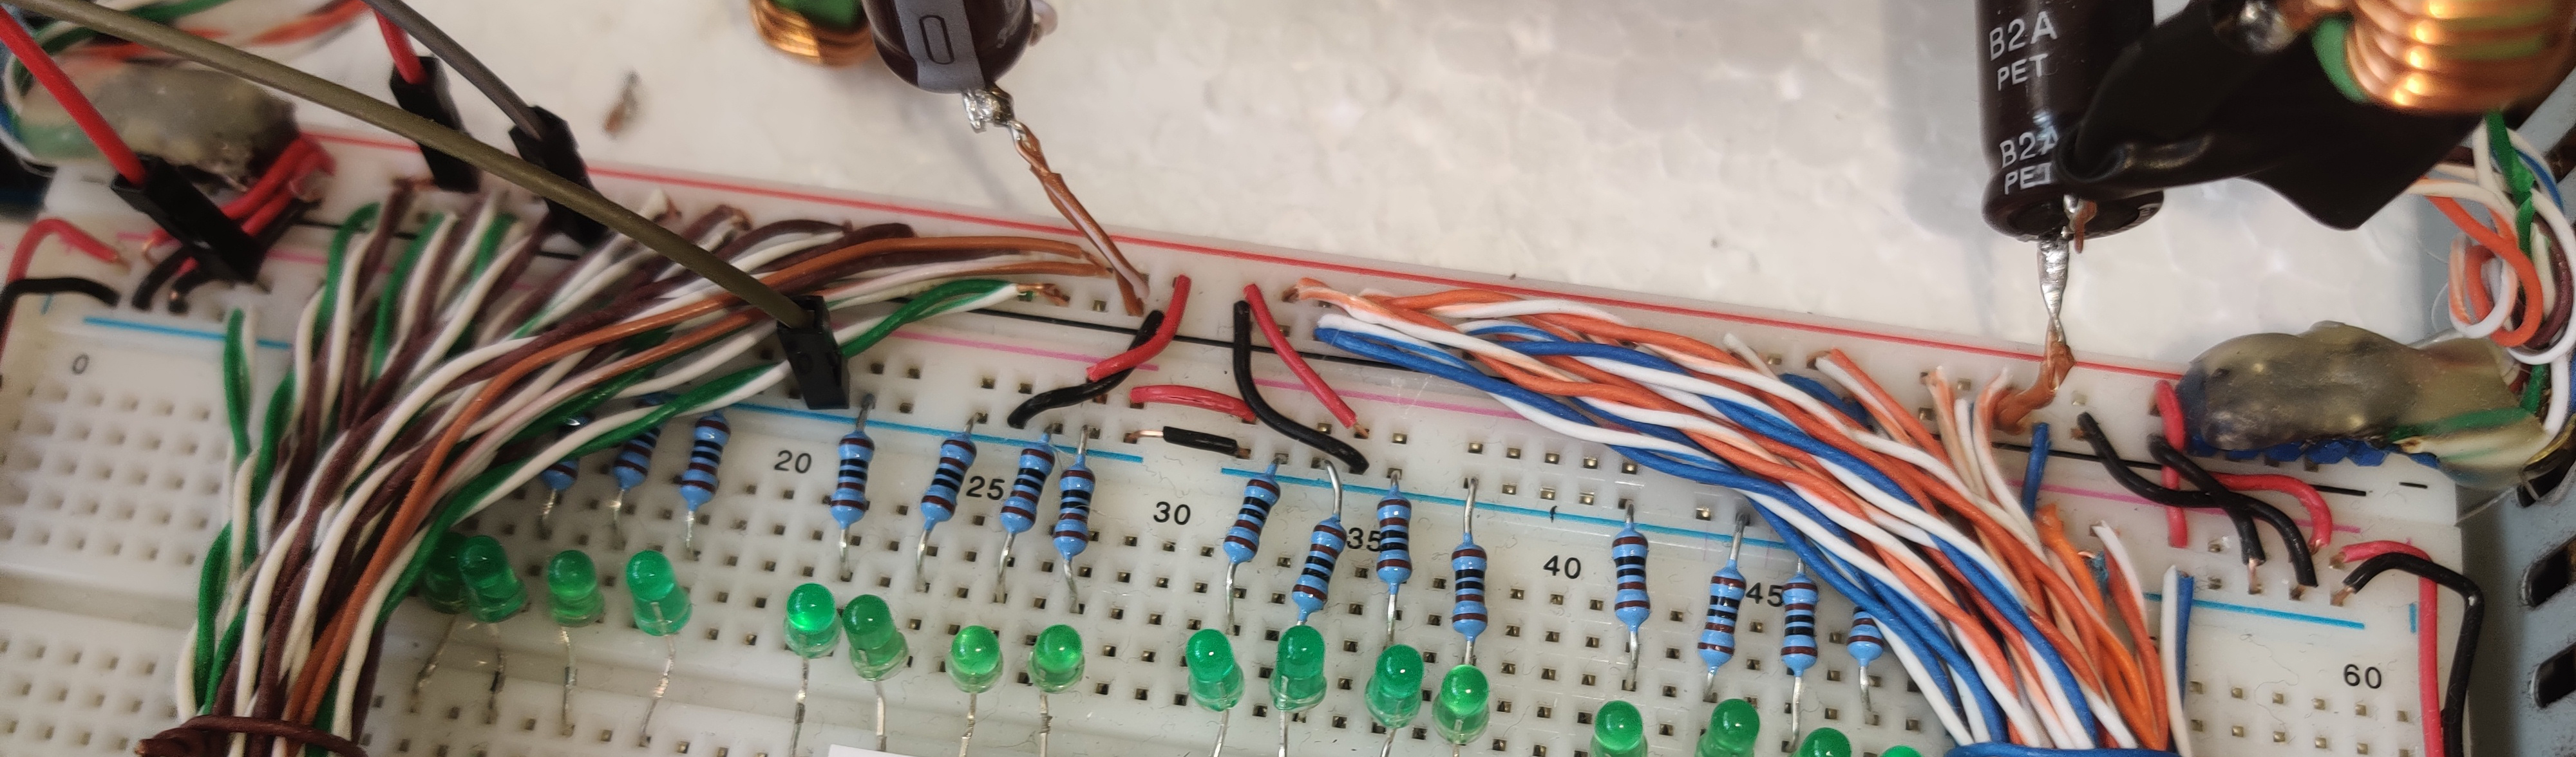
\includegraphics[scale=0.1]{power_strip}
  \caption{Power Strip connecting power cables from the salvadged ATX power connector}
  \label{power_strip}
\end{figure}

\begin{figure}[ht]
  \centering
  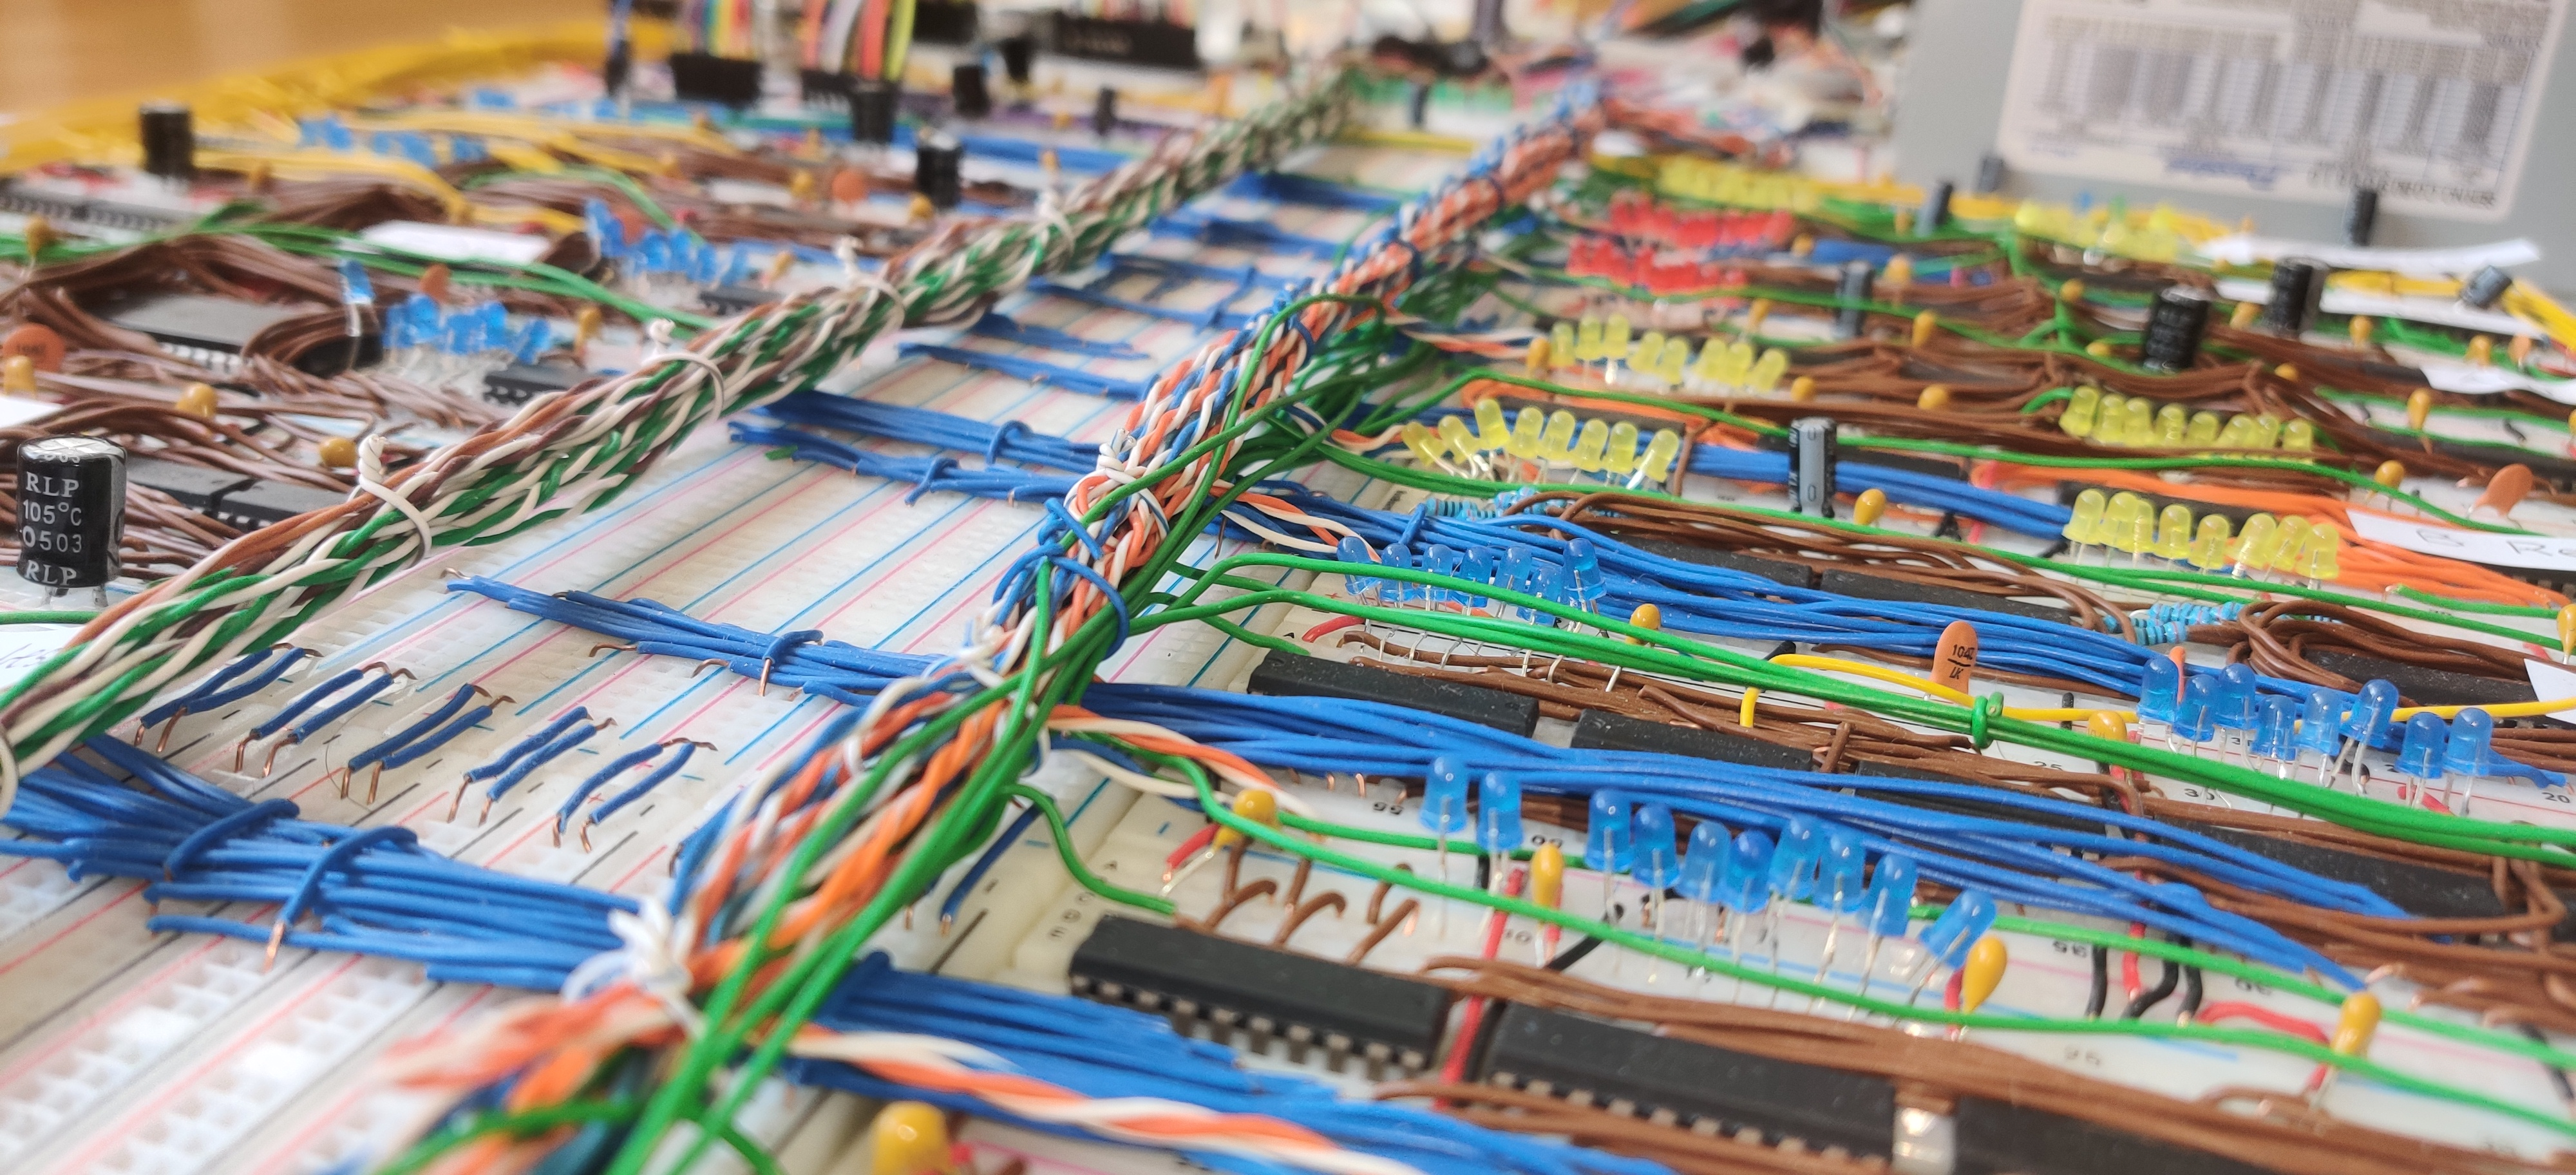
\includegraphics[scale=0.1]{power_conn}
  \caption{Power cable bundles spreading out across all breadboards}
  \label{power_conn}
\end{figure}


\subsection{Auxiliary Power Delivery}
Besides the main power delivery, there is another aspect which needs to be taken into account when
discussing adequate power delivery to all modules. An integrated circuit, when powered but not in
active use, draws a relatively stable amount of current. Whenever the circuit has an input change,
the transistors inside the circuit switch state. If many transistors switch state at
approximatively the same time, this can lead to noticable increases in momentary current draw. To
mitigate these current spikes, each chip is outfitted with a small 100 Nano-Farad ceramic
capacitor across its power and ground pins. These capacitors act like small batteries,
storing up charge when the circuit is stable and not drawing excessive power and then releasing
that charge when the current spikes occur. Besides the 100nF capacitors, larger capacitors were
desoldered from the motherboard from which the ATX power connector was harvested and then inserted
at regular intervals across the power strips of each modules \ref{cap}. These capaitors act just
like the smaller oanes, just at a larger scale, mitigating current spikes for multiple integrated
circuits at the same time.

\begin{figure}[ht]
  \centering
  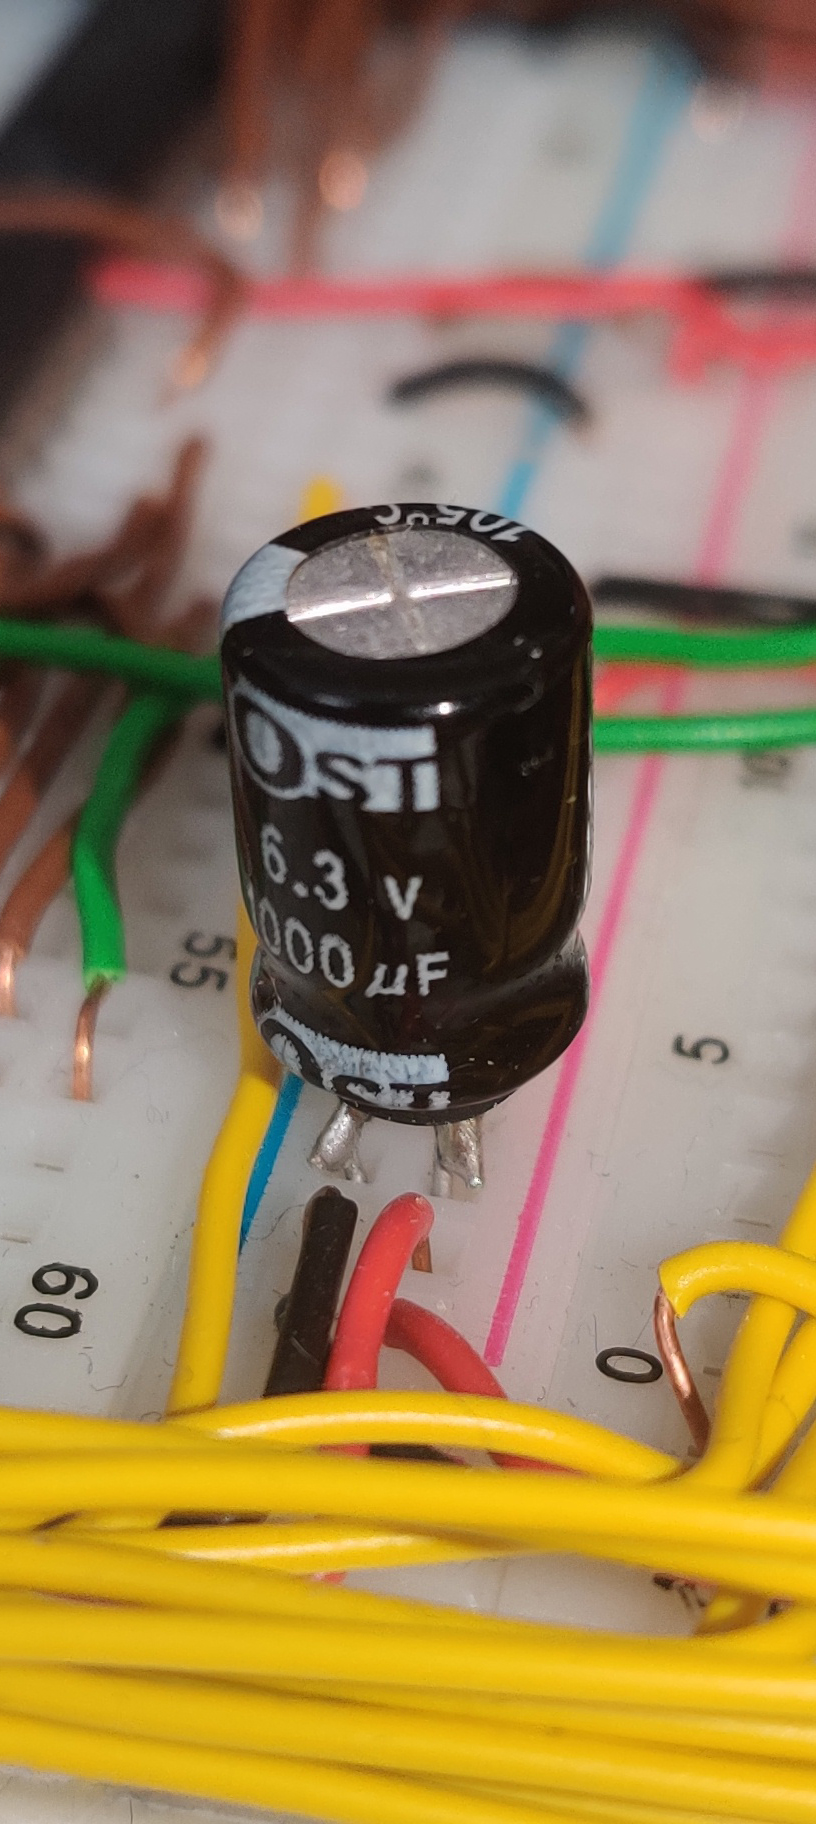
\includegraphics[scale=0.2]{cap}
  \caption{Power filter capacitor placed across breadboard power strips}
  \label{cap}
\end{figure}

\subsection{Sockets and Resistors}

\paragraph{Sockets}
There were to areas where the implementation of the 16-breadboard computer slightly deviated
from the schematics designs. First of all, \emph{Zero-Insertion-Force} (ZIF) Sockets were added
between the EEPROM chips on the control logic module \ref{socket}. These sockets use a small
lever to lock the pins of a chip in place. The chip is simply placed into the socket and then the
lever is pulled to tighten the chip in place. If the chip is to be removed from the socket, the
lever is pulled back and the chip can be removed without the need to apply any force (hence the
name ZIF). The reason why the sockets were used was that the EEPROM chips were to be removed and
re-inserted into the sockets many times, so as to re-program them with new or altered
instructions. This would have put a large strain on the breadboards, which could have led to
contact issues fairly quickly, an issue which would have been hard and time-consuming to debug.

\begin{figure}[ht]
  \centering
  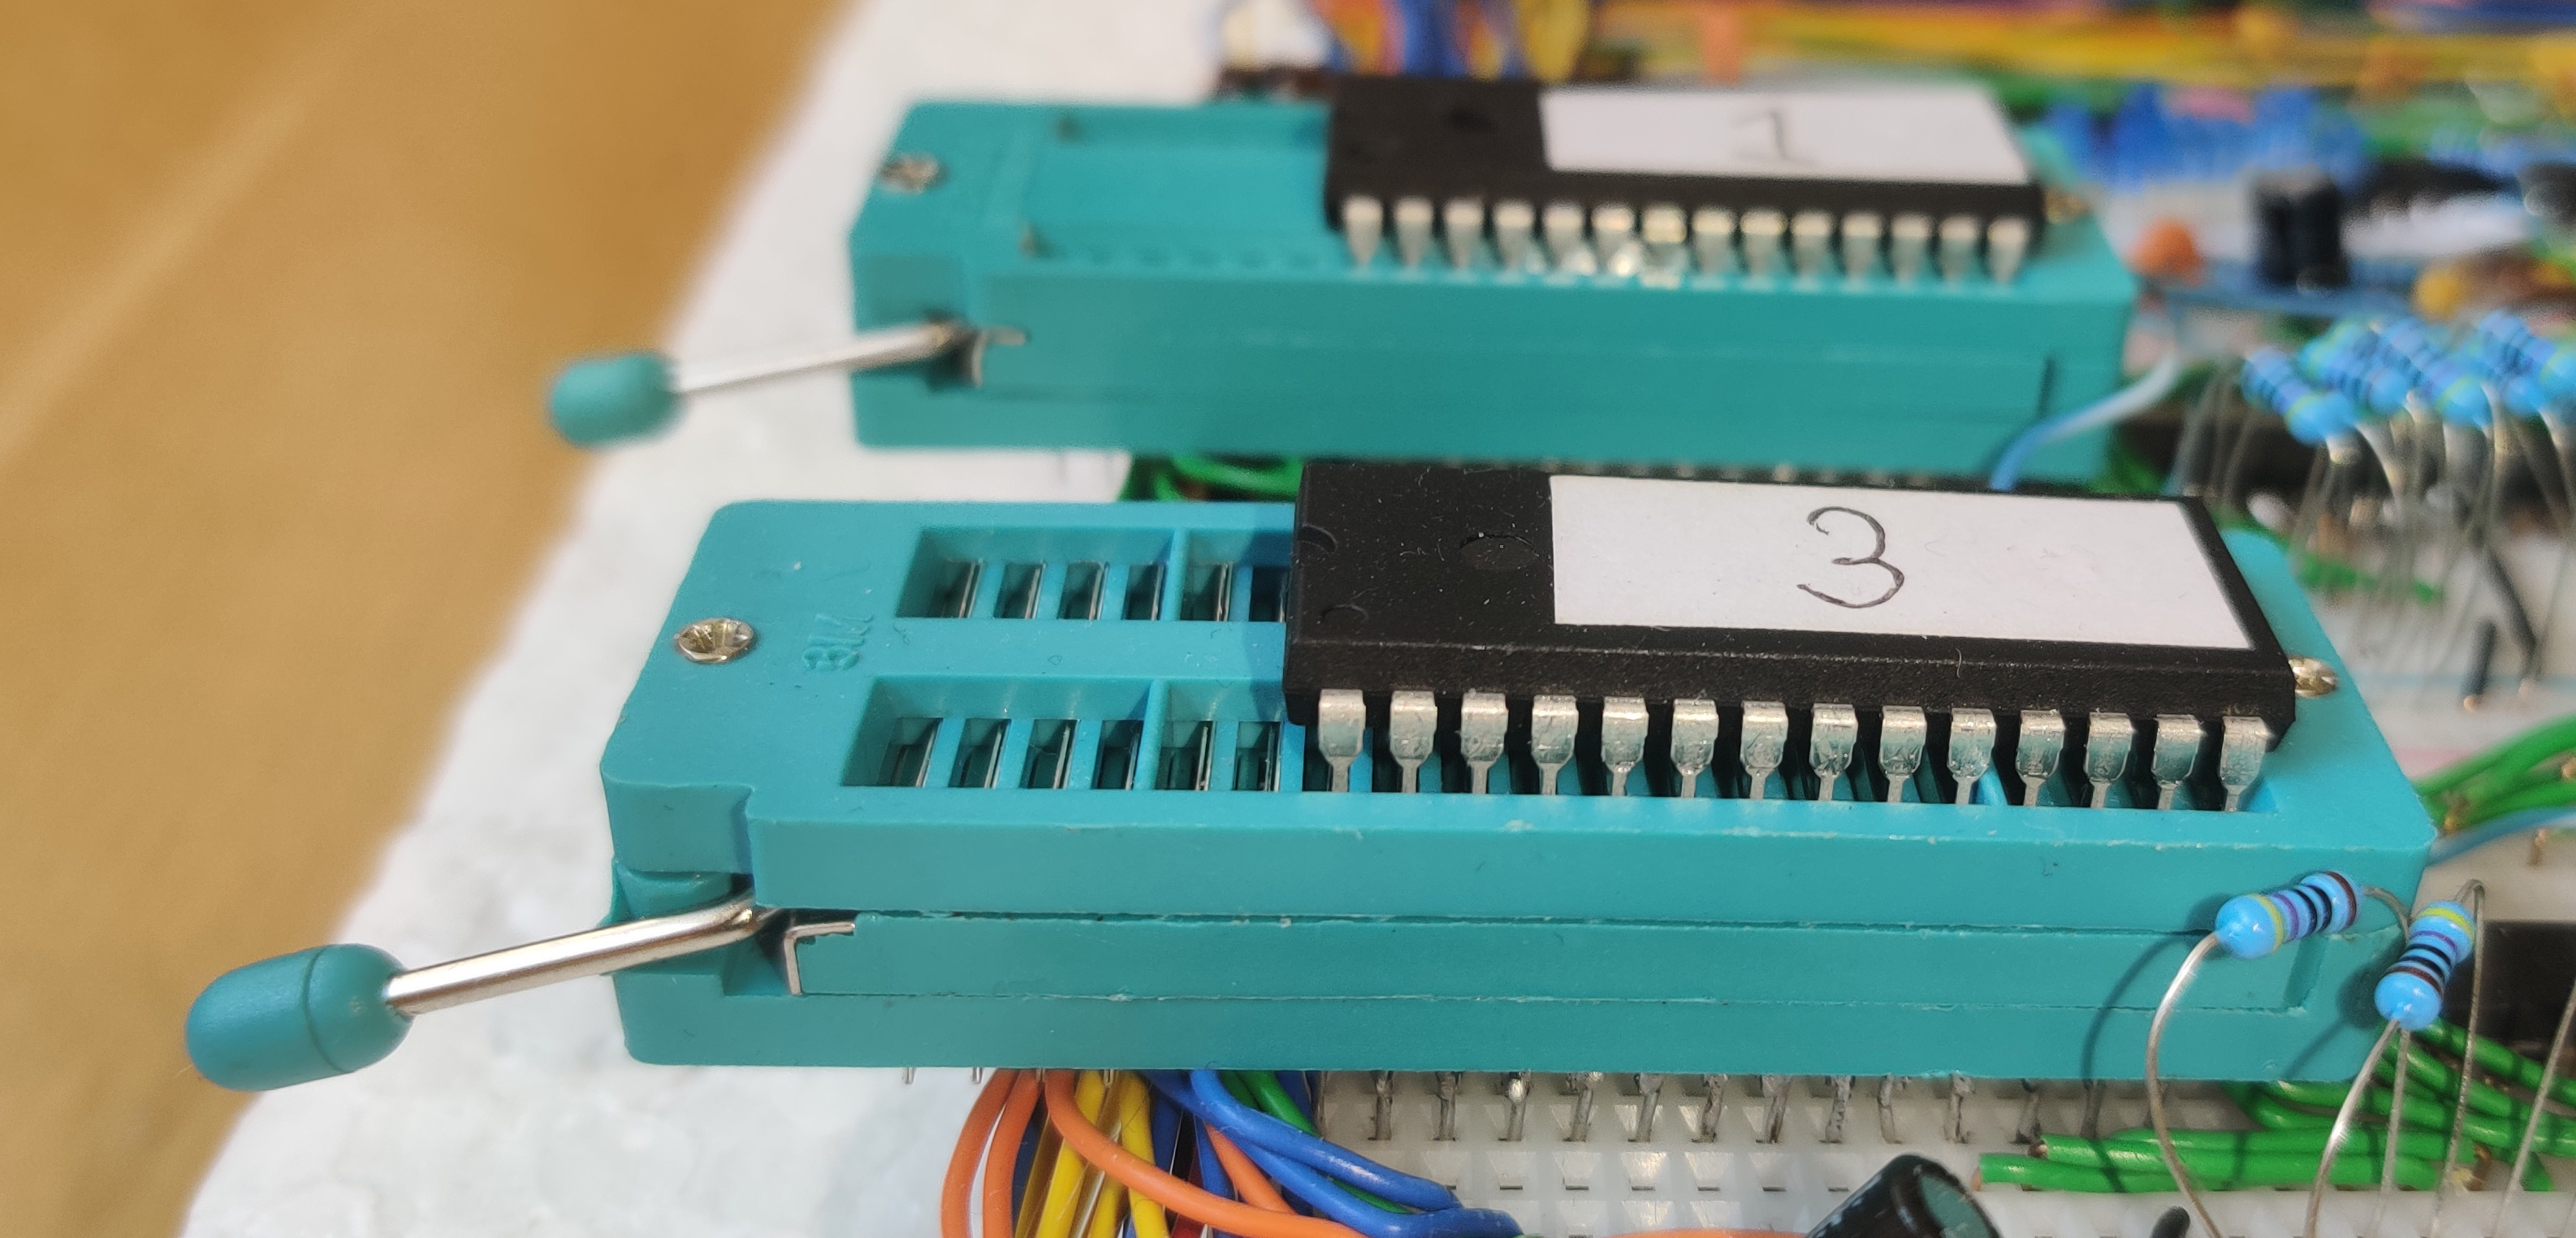
\includegraphics[scale=0.1]{socket}
  \caption{AT28C64B \cite{at28c64b} EEPROM chips inserted into \emph{ZIF} sockets}
  \label{socket}
\end{figure}


 \paragraph{Resistors}
 Normally when installing an LED, it is important to use a resistor in series between the LED
 and either the ground or the voltage lead. This prevents the LED from drawing too much current
 and burning up. In many instances across multiple modules, there was not enough space on the
 breadboards to fit both LEDs and resistors. As such, in those ares the resistor was not
 installed and instead the LED was connected directy between the voltage source and the ground
 lead. While this is definetly bad practice and it was avoided as much as possible, this
 compromise ws made where necessary because the LEDs were always connected to a chip output and
 not to the 5V rail directly. The chips from the \emph{74LS} family have a very limited maximum
 ouput current. This current was not high enough to burn up the LED. As such, the LEDs could
 be connected directly to the chips and then to Ground without the fear of having them burn up.
 This was not without consequences though. The small maximum output current of the \emph{74LS}
 chips was still larger than if it would have been limited through a resistor. As such, the
 overall current draw of the computer increased. Given the robust power solution put in place,
 this didn't cause any issues.

 \section{Hardware Implementation Tools}
 Since the breadboards don't require solder to form connections, very few tools are actually
 needed to build on them. A pair of pliers and side cutters were used to cut off the isolation
 on the ends of wires to form pins which can then be inserted into the breadboard. In case it is
 availalbe, a wire stripper can also be used instead. It would be preffered, since a wire cutter
 is much more reliable at producing equally sized pins.
 A small flat-head screwdriver can be used to extract wires and chips which have been wrongly
 positioned. The breadboards come preapplied with an adhesive backing. To separate the breadboards
 from the power strips, a cutter was used to cut through this backing.
 An a few occasions, a soldering iron and solder was needed (for example to extract components
 from the donor motherboard). Finally, a multimeter was used to ensure that connections have been
 made correctly and to measure voltages.

 \section{Implementation process for one module}
The implementation process for a 16-bit breadboard computer modules is straight forward and easy
to follow.
\begin{enumerate}
  \item Ensure all needed tools and components (breadboards/ICs/wires/capaitors/LEDs) are at
  hand, as well as the design schematic for that particular module
  \item Lay out the chips on the breadboard
  \item Based on the connections made in the schematic, measure out wires to connect the pins of
  the different integrated circuits
  \item cut the wires to that length, plus an added centimeter for the two pins, then strip out
  5 milimeters of insulation off of each end to form the pins
  \item connect the wires to the breadboard
  \item plug the LEDs and Capacitors into the breadboard
  \item Connect and label control signals going into and out of the module
\end{enumerate}

\section{Physical implementation}
The process outlined previously process was followed thoroughly for each module of the 16-bit
breadboard computer. The modules were built in the following order:
\begin{enumerate}
  \item \textbf{Clock Module} \ref{clock-i}
  \item \textbf{A Register} \ref{a-reg-i}
  \item \textbf{B Register} \ref{b-reg-i}
  \item \textbf{C Register} \ref{c-reg-i}
  \item \textbf{Instruction Register} \ref{ir-i}
  \item \textbf{Memory Address Register} \ref{mar-i}
  \item \textbf{Flags Register} \ref{flags-i}
  \item \textbf{I/O} \ref{io-i}
  \item \textbf{ALU} \ref{alu-i}
  \item \textbf{Shift Register} \ref{shift-reg-i}
  \item \textbf{Program Counter} \ref{pc-i}
  \item \textbf{Stack Pointer} \ref{sp-i}
  \item \textbf{Word Selector} \ref{word-select-i}
  \item \textbf{Address Selector} \ref{addr-select-i}
  \item \textbf{RAM} \ref{ram}
  \item \textbf{Display} \ref{display}
  \item \textbf{Control Signals} \ref{control-sigs-i}
  \item \textbf{Control Logic} \ref{control-logic-i}
  \item \textbf{High level overview (with bus and LEDs visible)} \ref{high-level-i}
\end{enumerate}


  \begin{figure}[h]
    \centering
    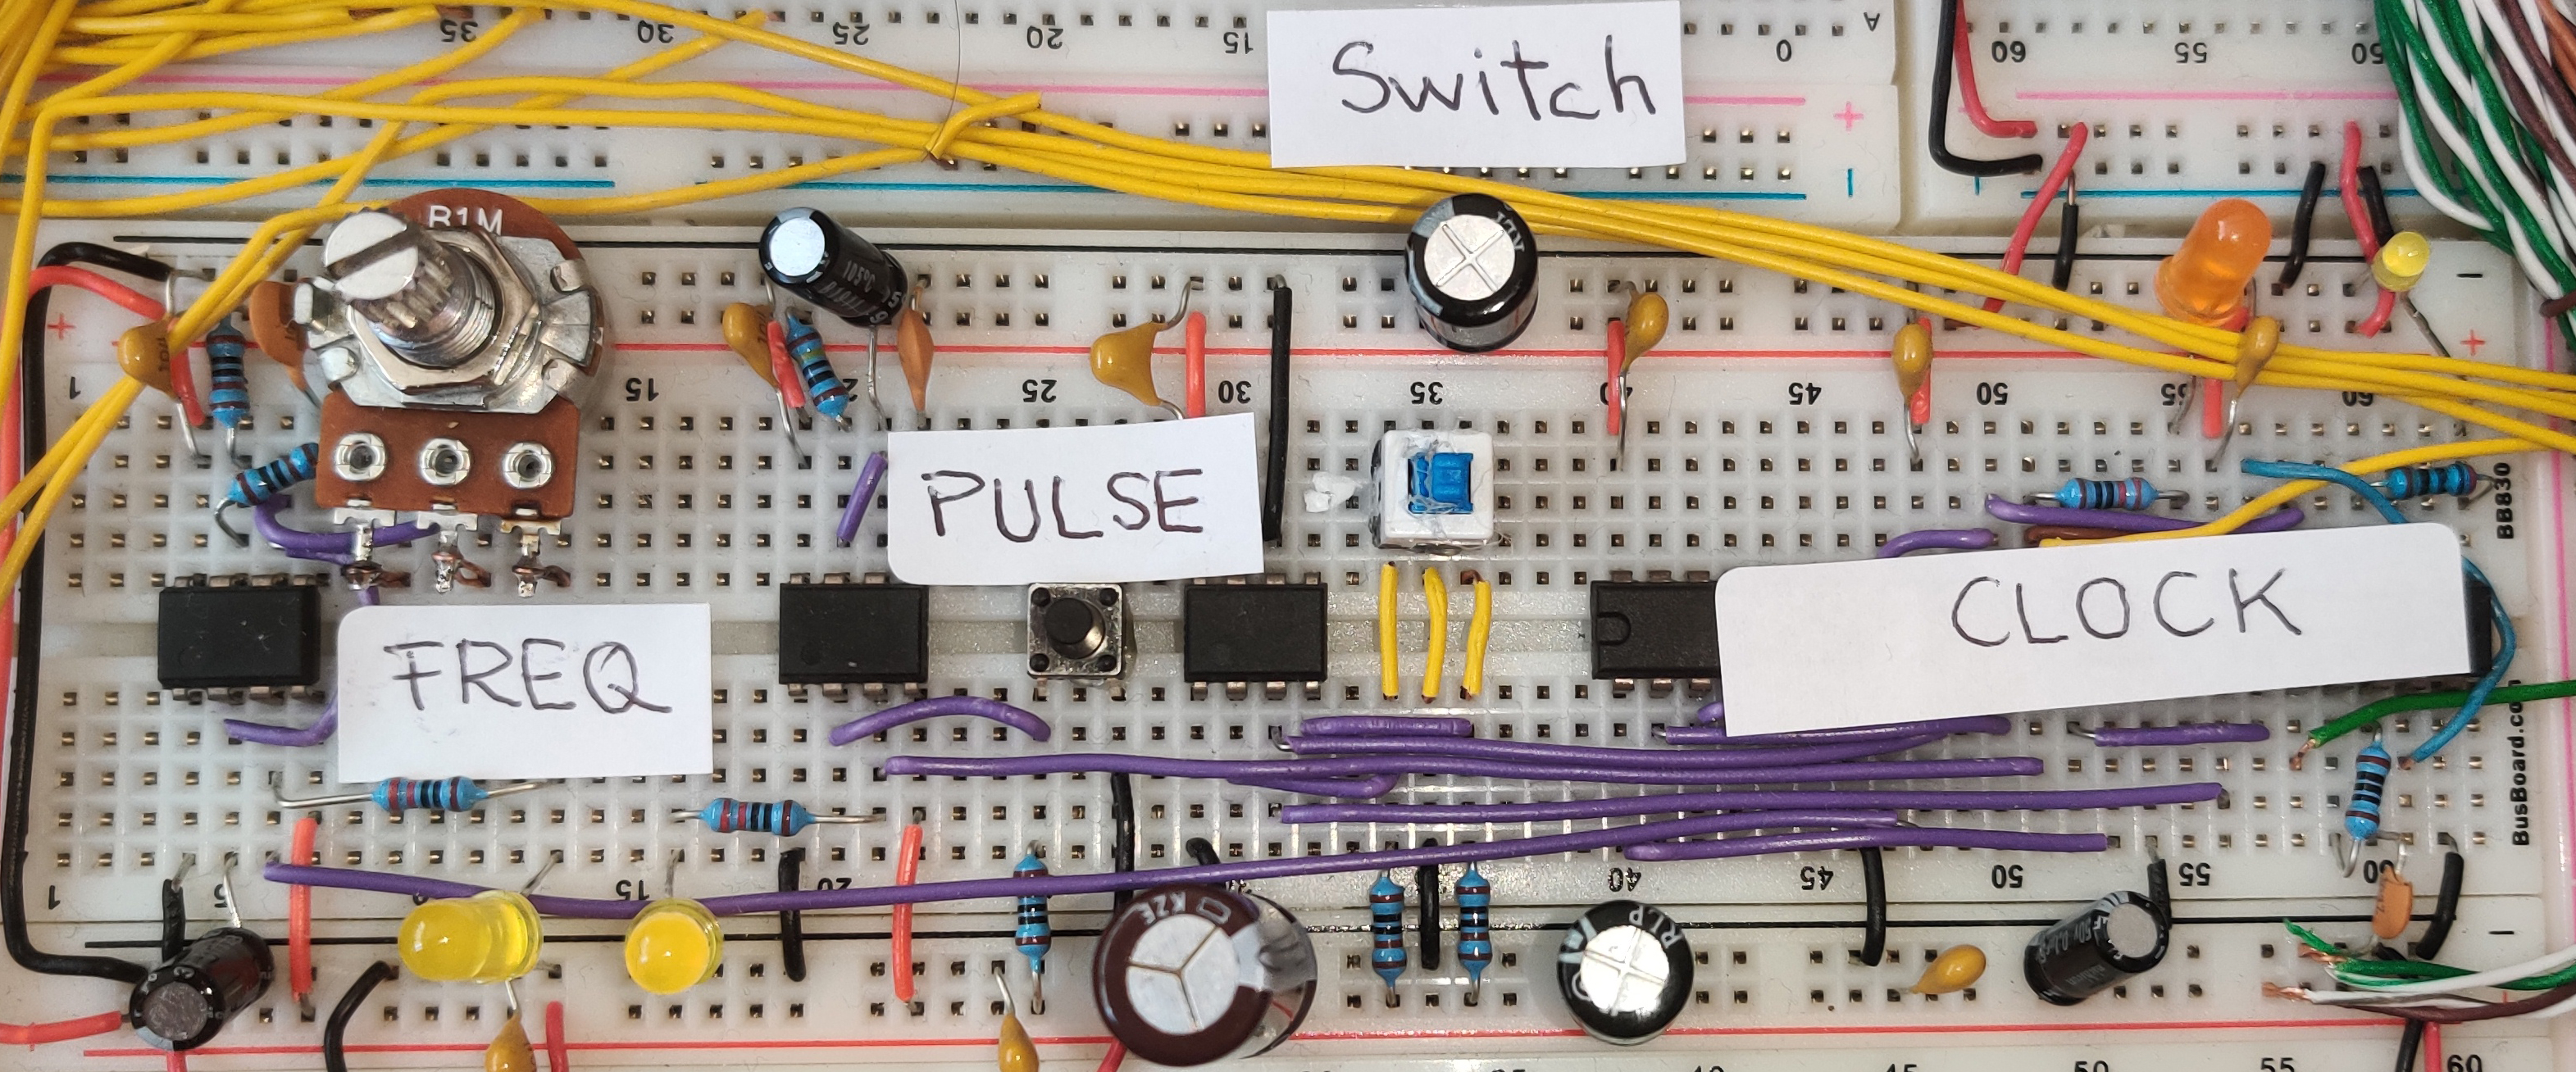
\includegraphics[scale=0.1]{comp/clock}
    \caption{Clock implementation}
    \label{clock-i}
  \end{figure}

  \begin{figure}[h]
    \centering
    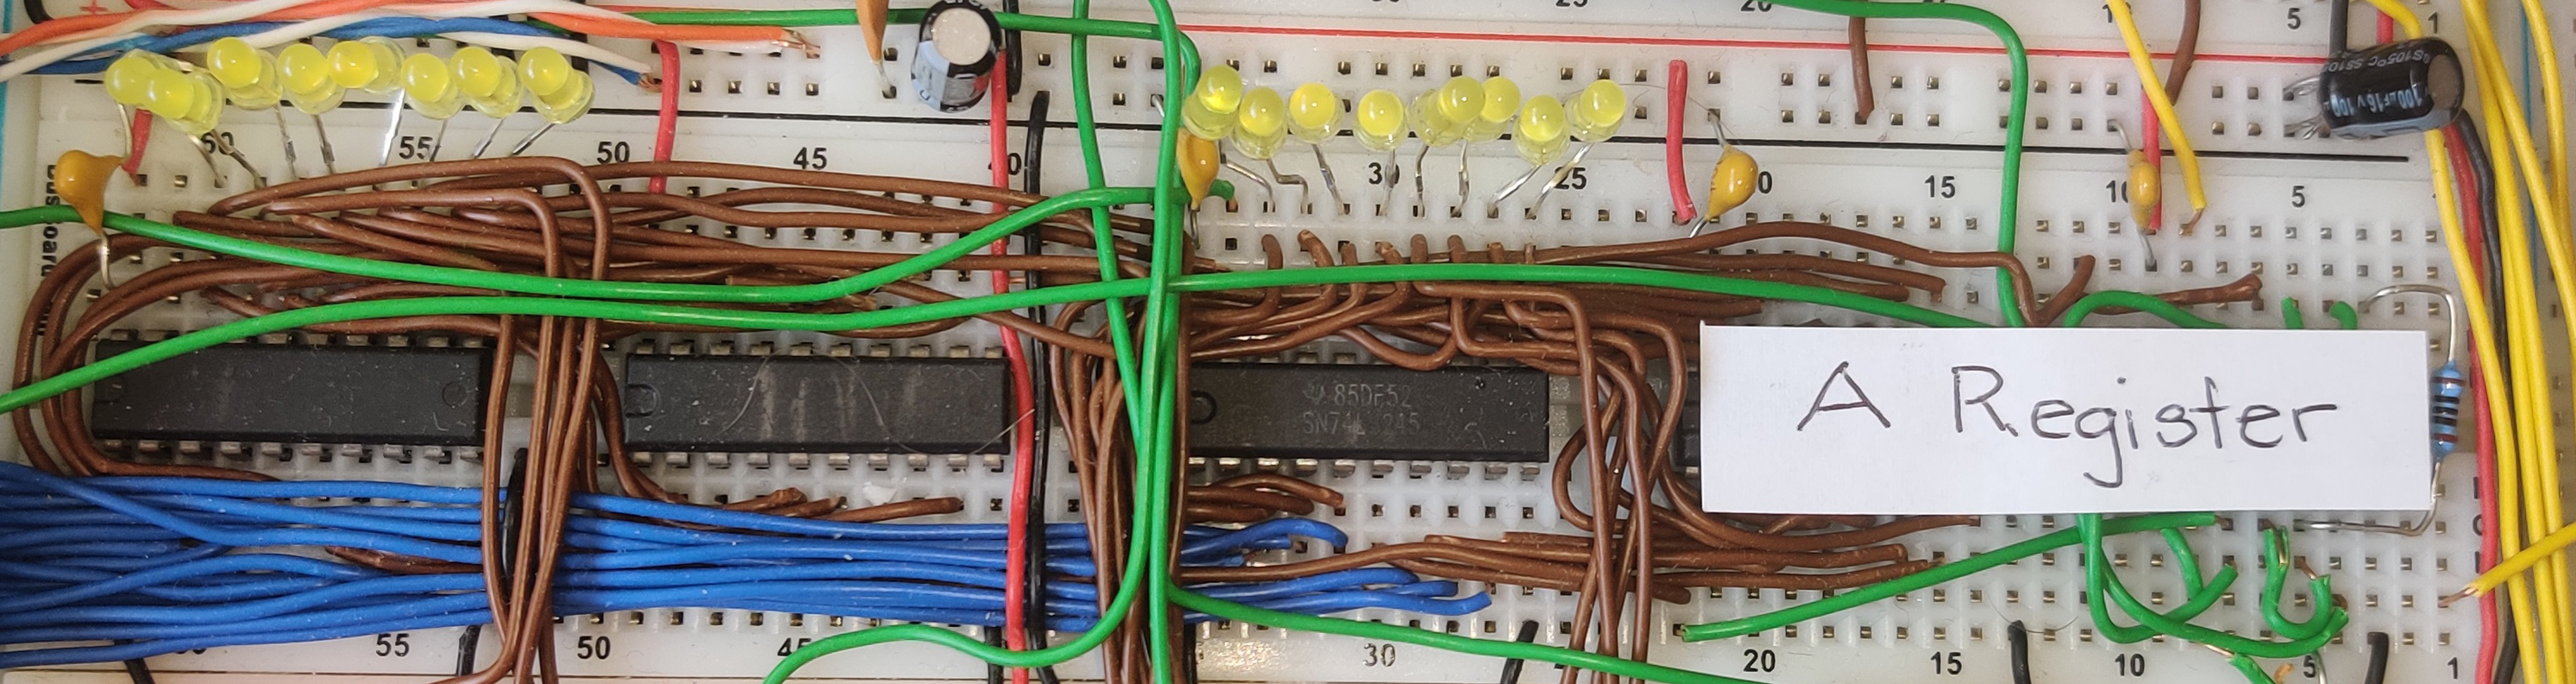
\includegraphics[scale=0.1]{comp/a-reg}
    \caption{A register implementation}
    \label{a-reg-i}
  \end{figure}

  \begin{figure}[h]
    \centering
    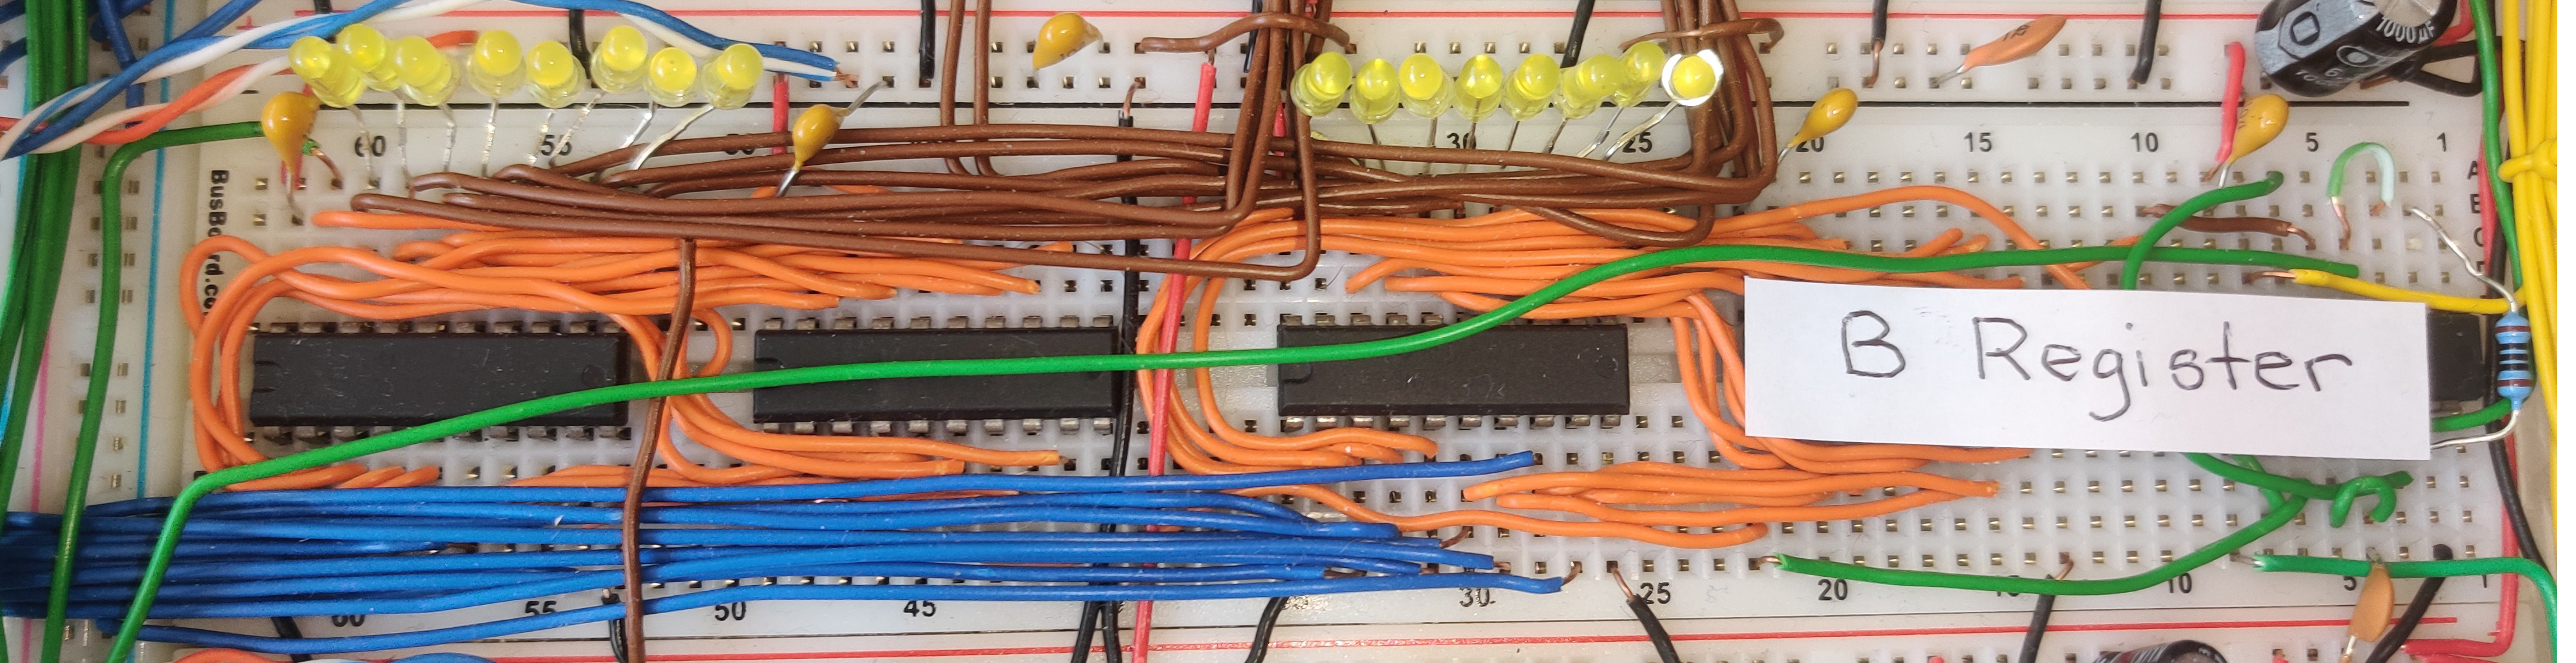
\includegraphics[scale=0.1]{comp/b-reg}
    \caption{B register implementation}
    \label{b-reg-i}
  \end{figure}

  \begin{figure}[h]
    \centering
    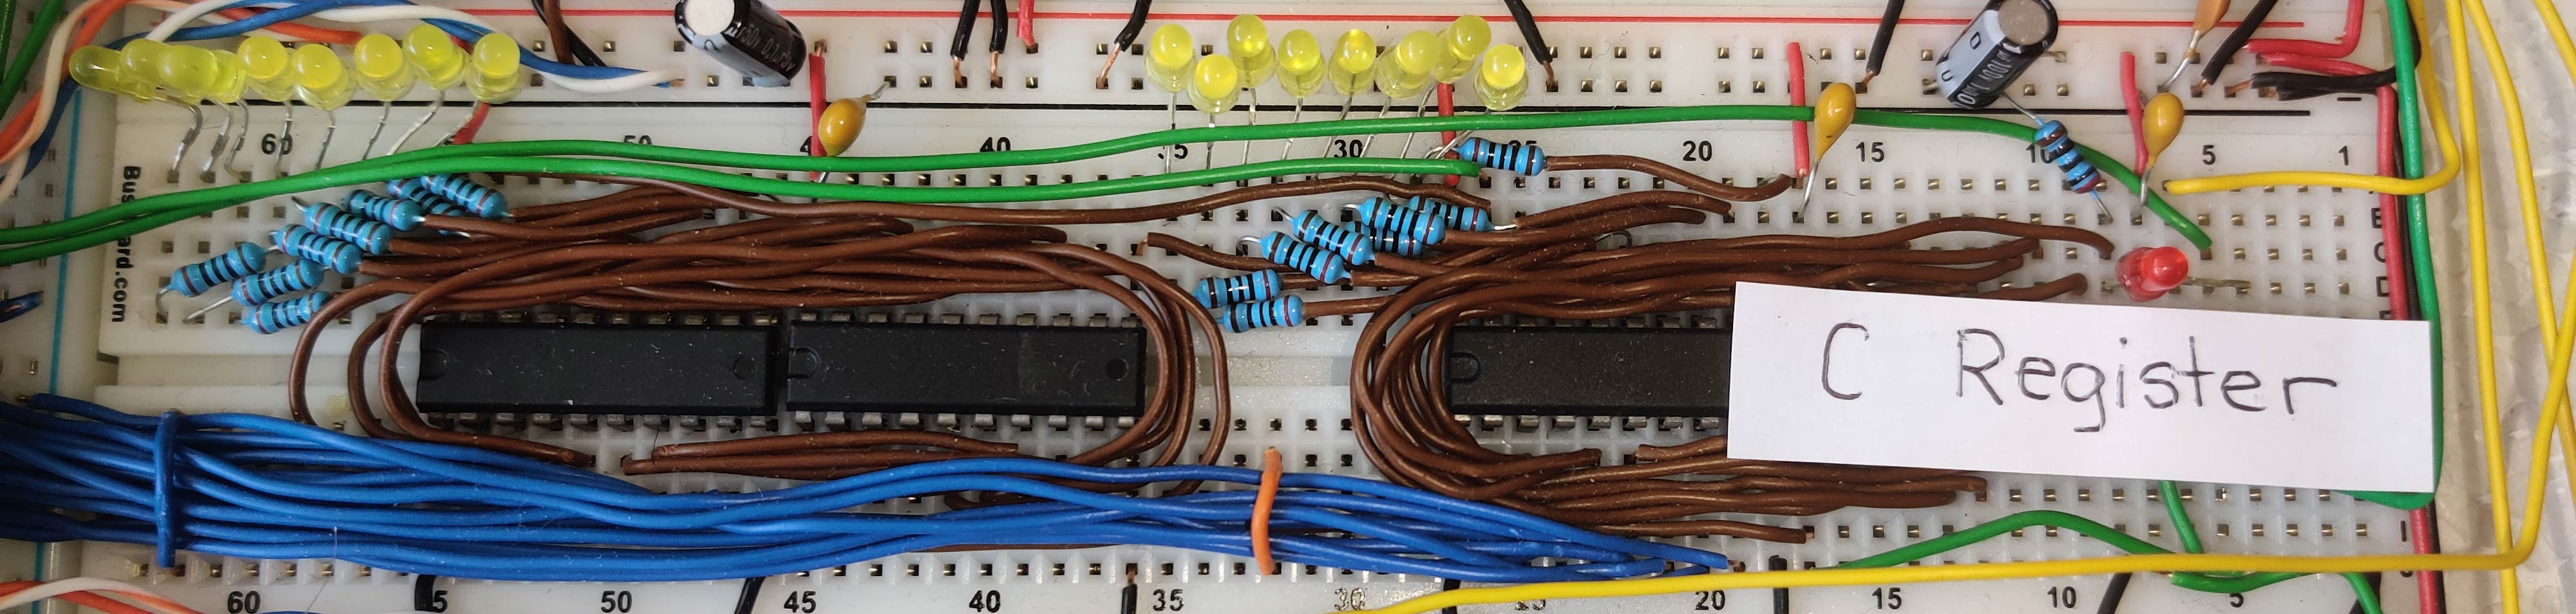
\includegraphics[scale=0.1]{comp/c-reg}
    \caption{C register implementation}
    \label{c-reg-i}
  \end{figure}

  \begin{figure}[h]
    \centering
    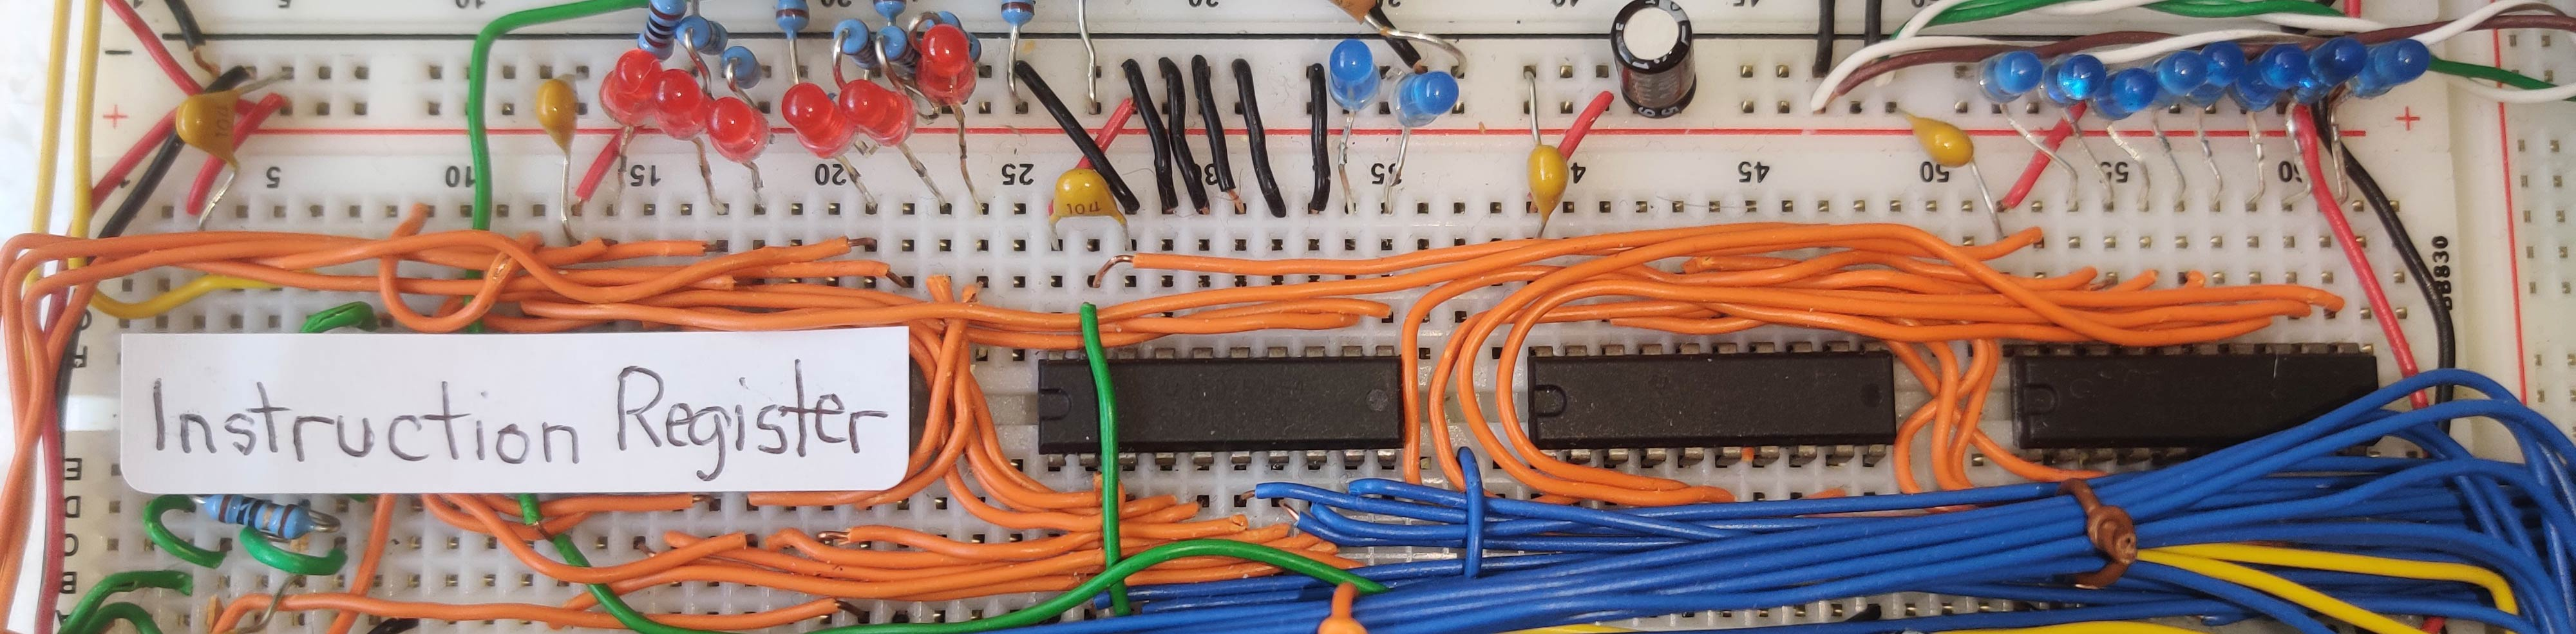
\includegraphics[scale=0.1]{comp/ir}
    \caption{Instruction register implementation}
    \label{ir-i}
  \end{figure}

  \begin{figure}[h]
    \centering
    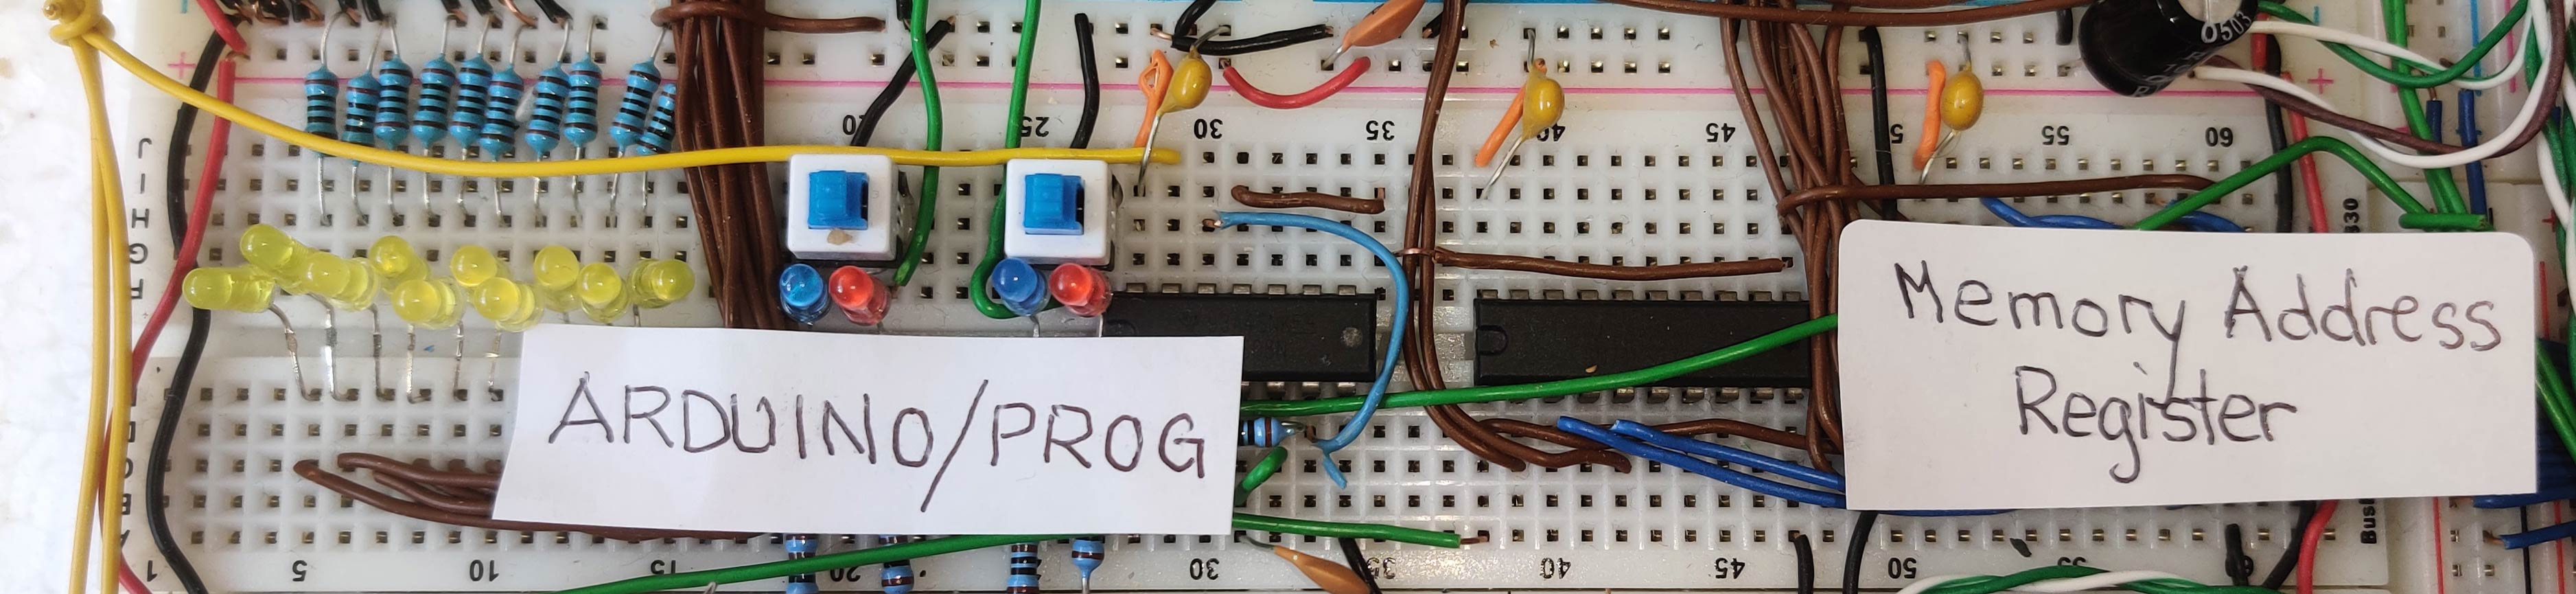
\includegraphics[scale=0.1]{comp/mar}
    \caption{Memory address register implementation}
    \label{mar-i}
  \end{figure}

  \begin{figure}[h]
    \centering
    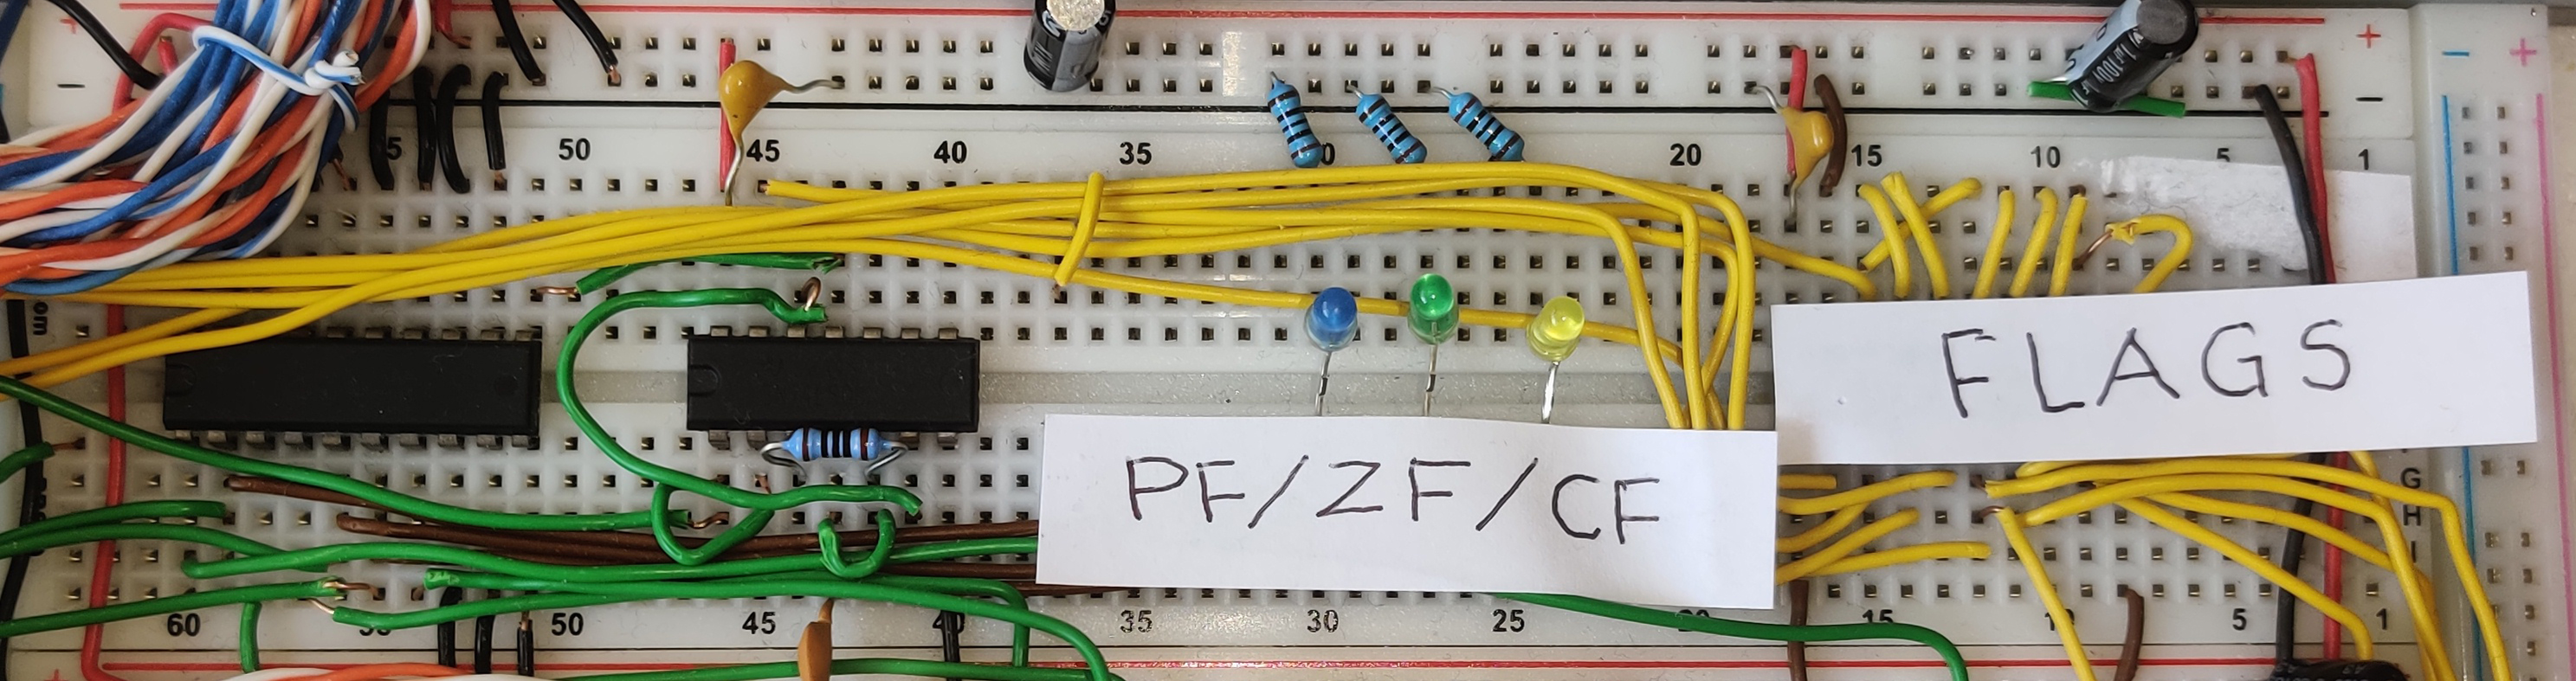
\includegraphics[scale=0.1]{comp/flags}
    \caption{Flags register implementation}
    \label{flags-i}
  \end{figure}

  \begin{figure}[h]
    \centering
    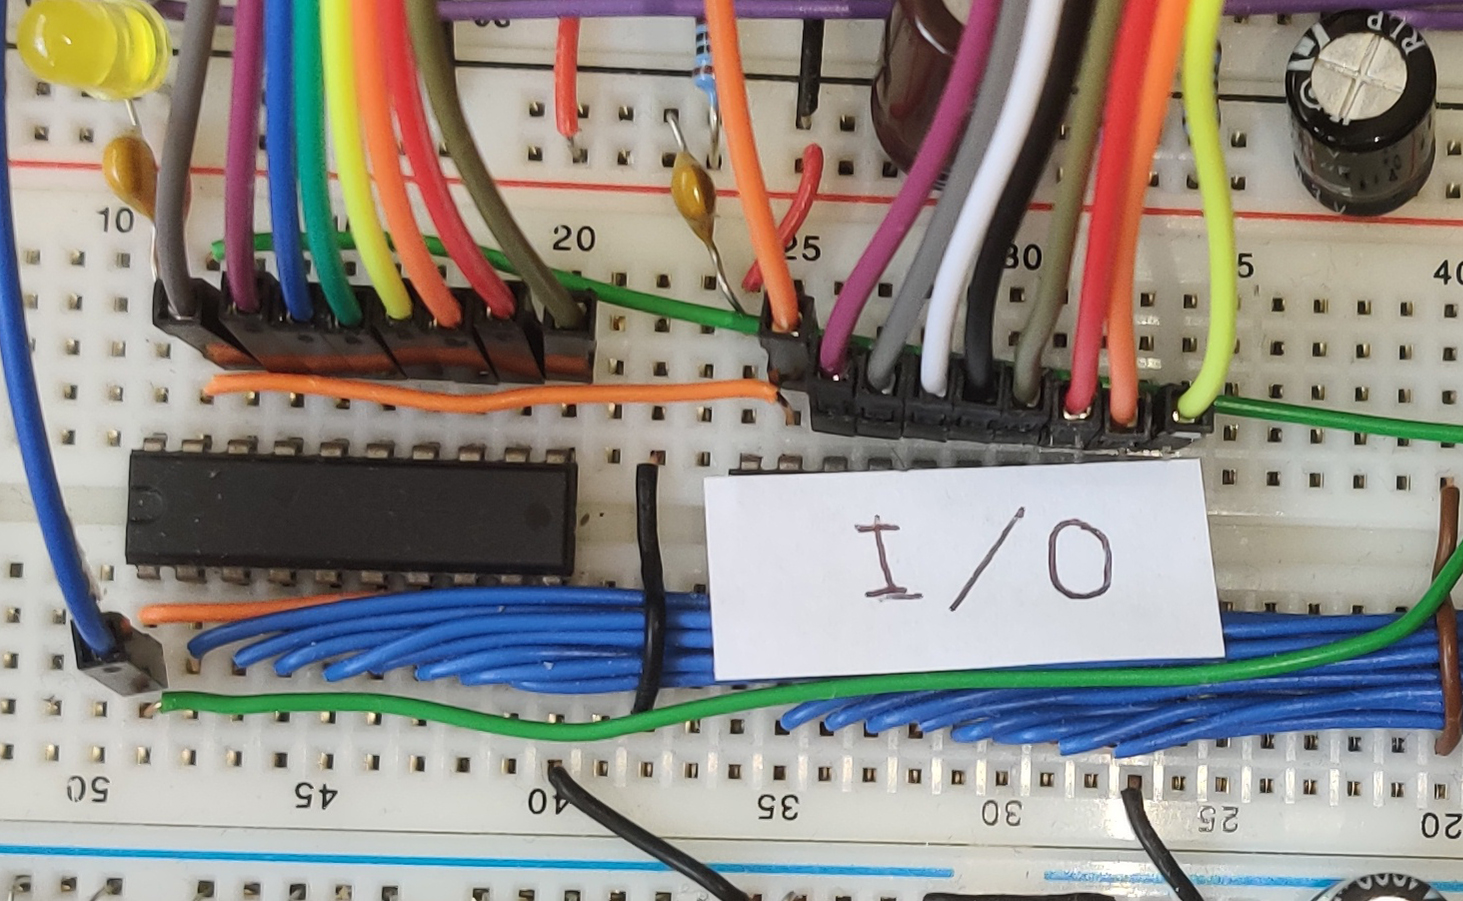
\includegraphics[scale=0.1]{comp/io}
    \caption{Input/Output implementation}
    \label{io-i}
  \end{figure}

  \begin{figure}[h]
    \centering
    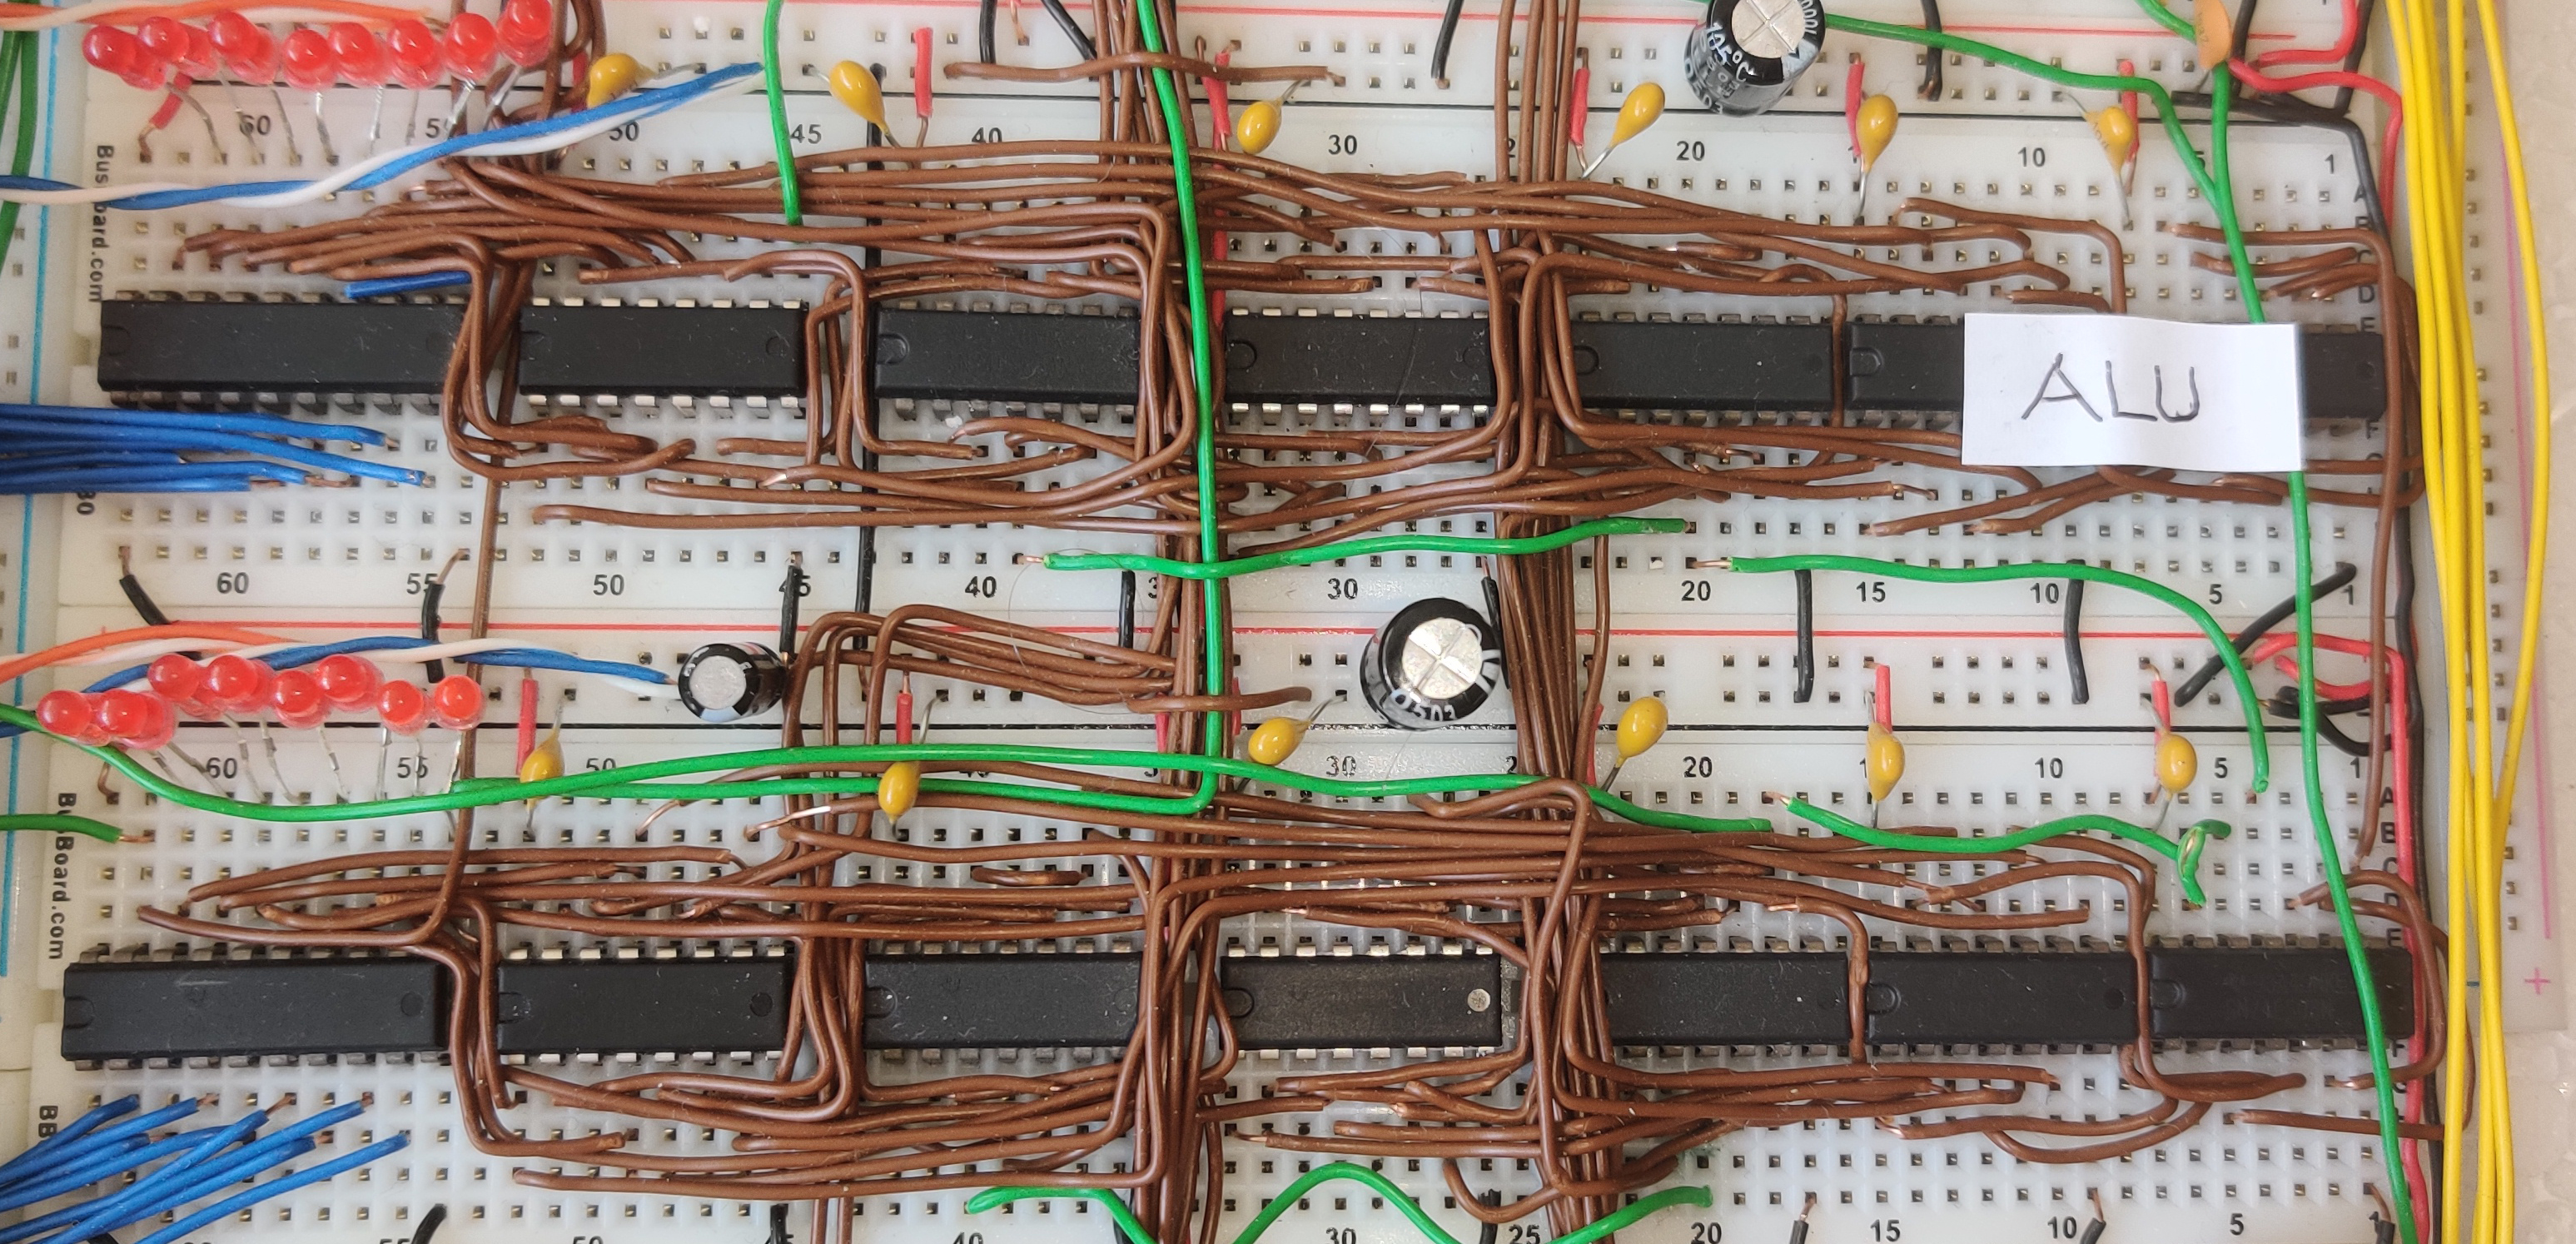
\includegraphics[scale=0.1]{comp/alu}
    \caption{Arithmetic-Logic Unit implementation}
    \label{alu-i}
  \end{figure}

  \begin{figure}[h]
    \centering
    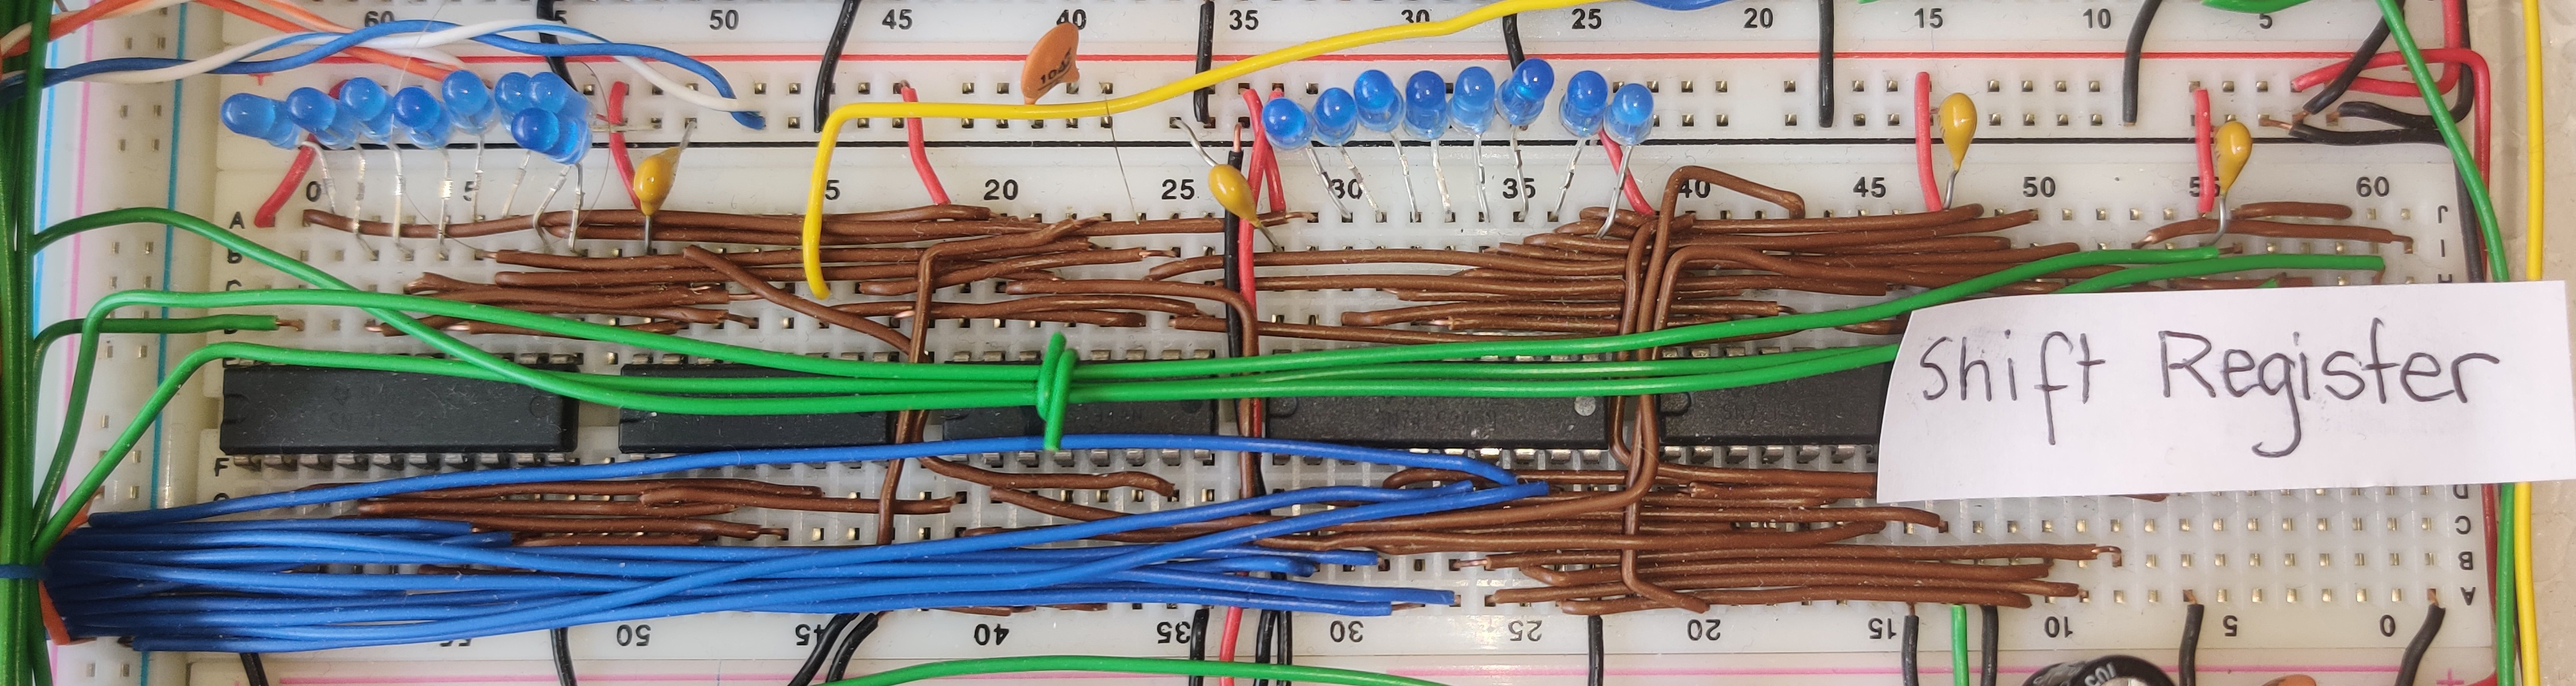
\includegraphics[scale=0.1]{comp/shift-reg}
    \caption{Shift Register implementation}
    \label{shift-reg-i}
  \end{figure}

  \begin{figure}[h]
    \centering
    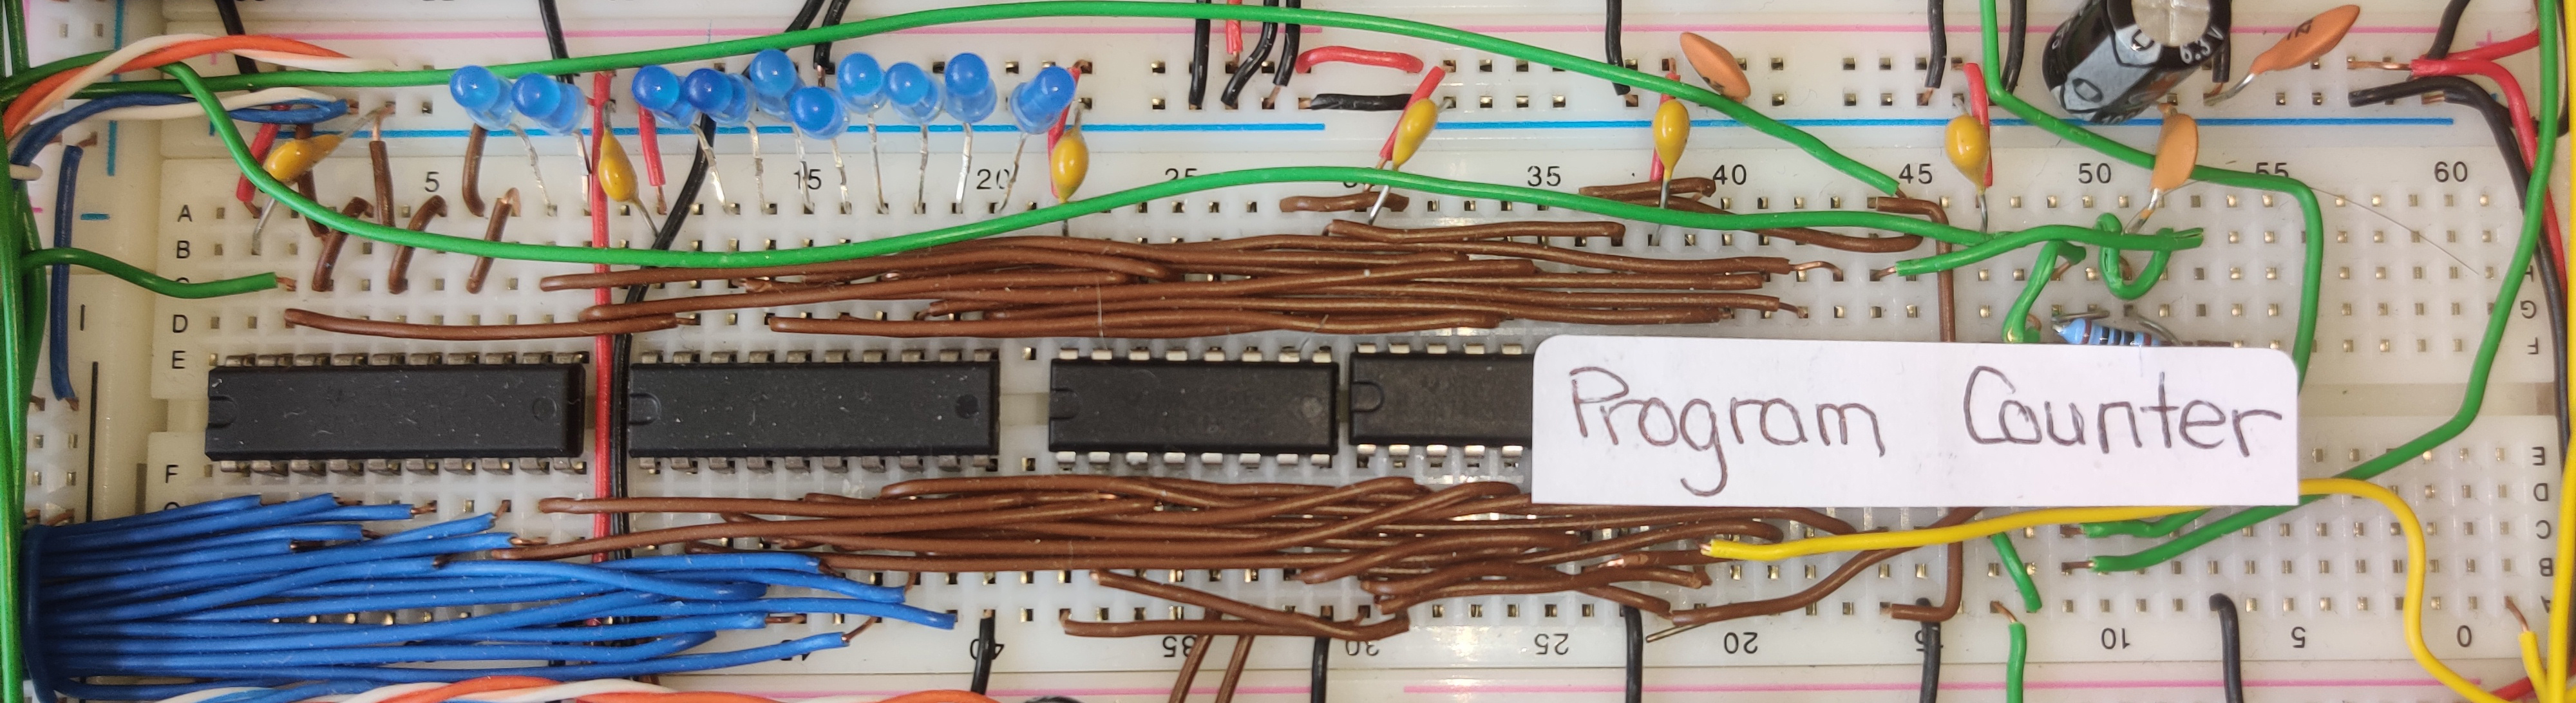
\includegraphics[scale=0.1]{comp/pc}
    \caption{Program Counter implementation}
    \label{pc-i}
  \end{figure}

  \begin{figure}[h]
    \centering
    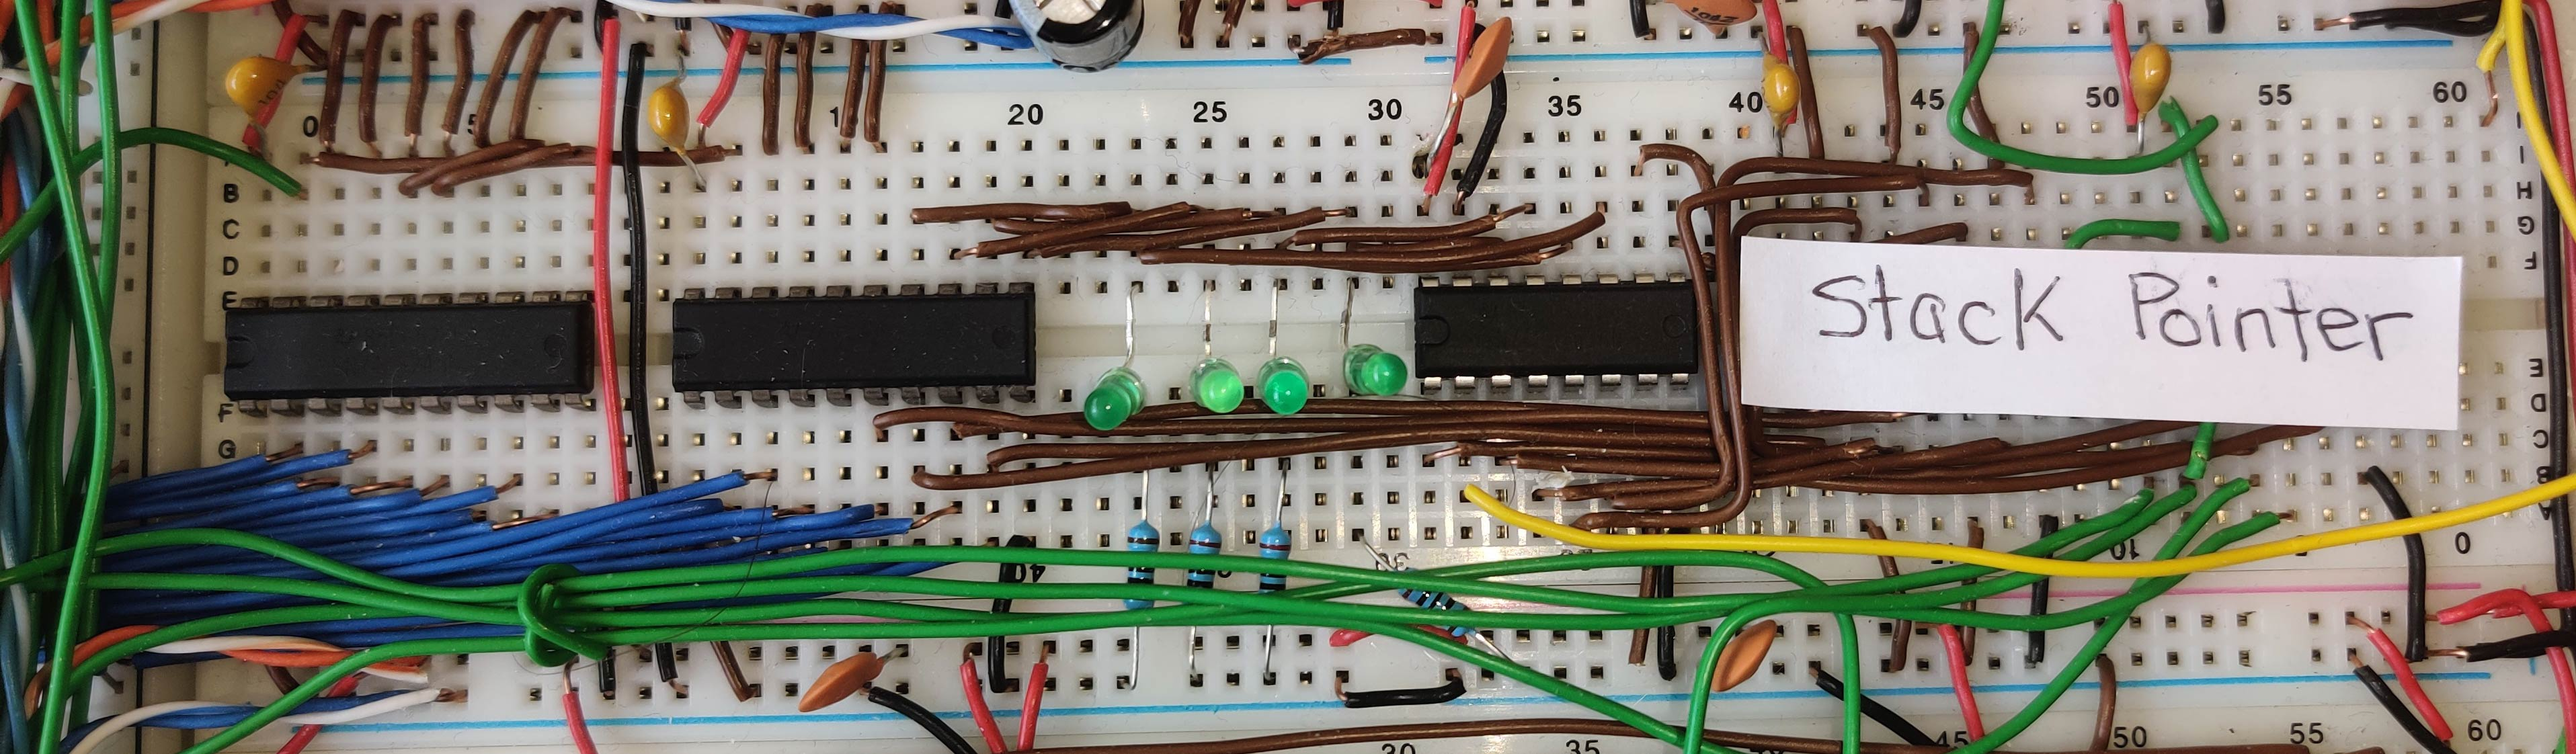
\includegraphics[scale=0.1]{comp/sp}
    \caption{Stack Pointer implementation}
    \label{sp-i}
  \end{figure}

  \begin{figure}[h]
    \centering
    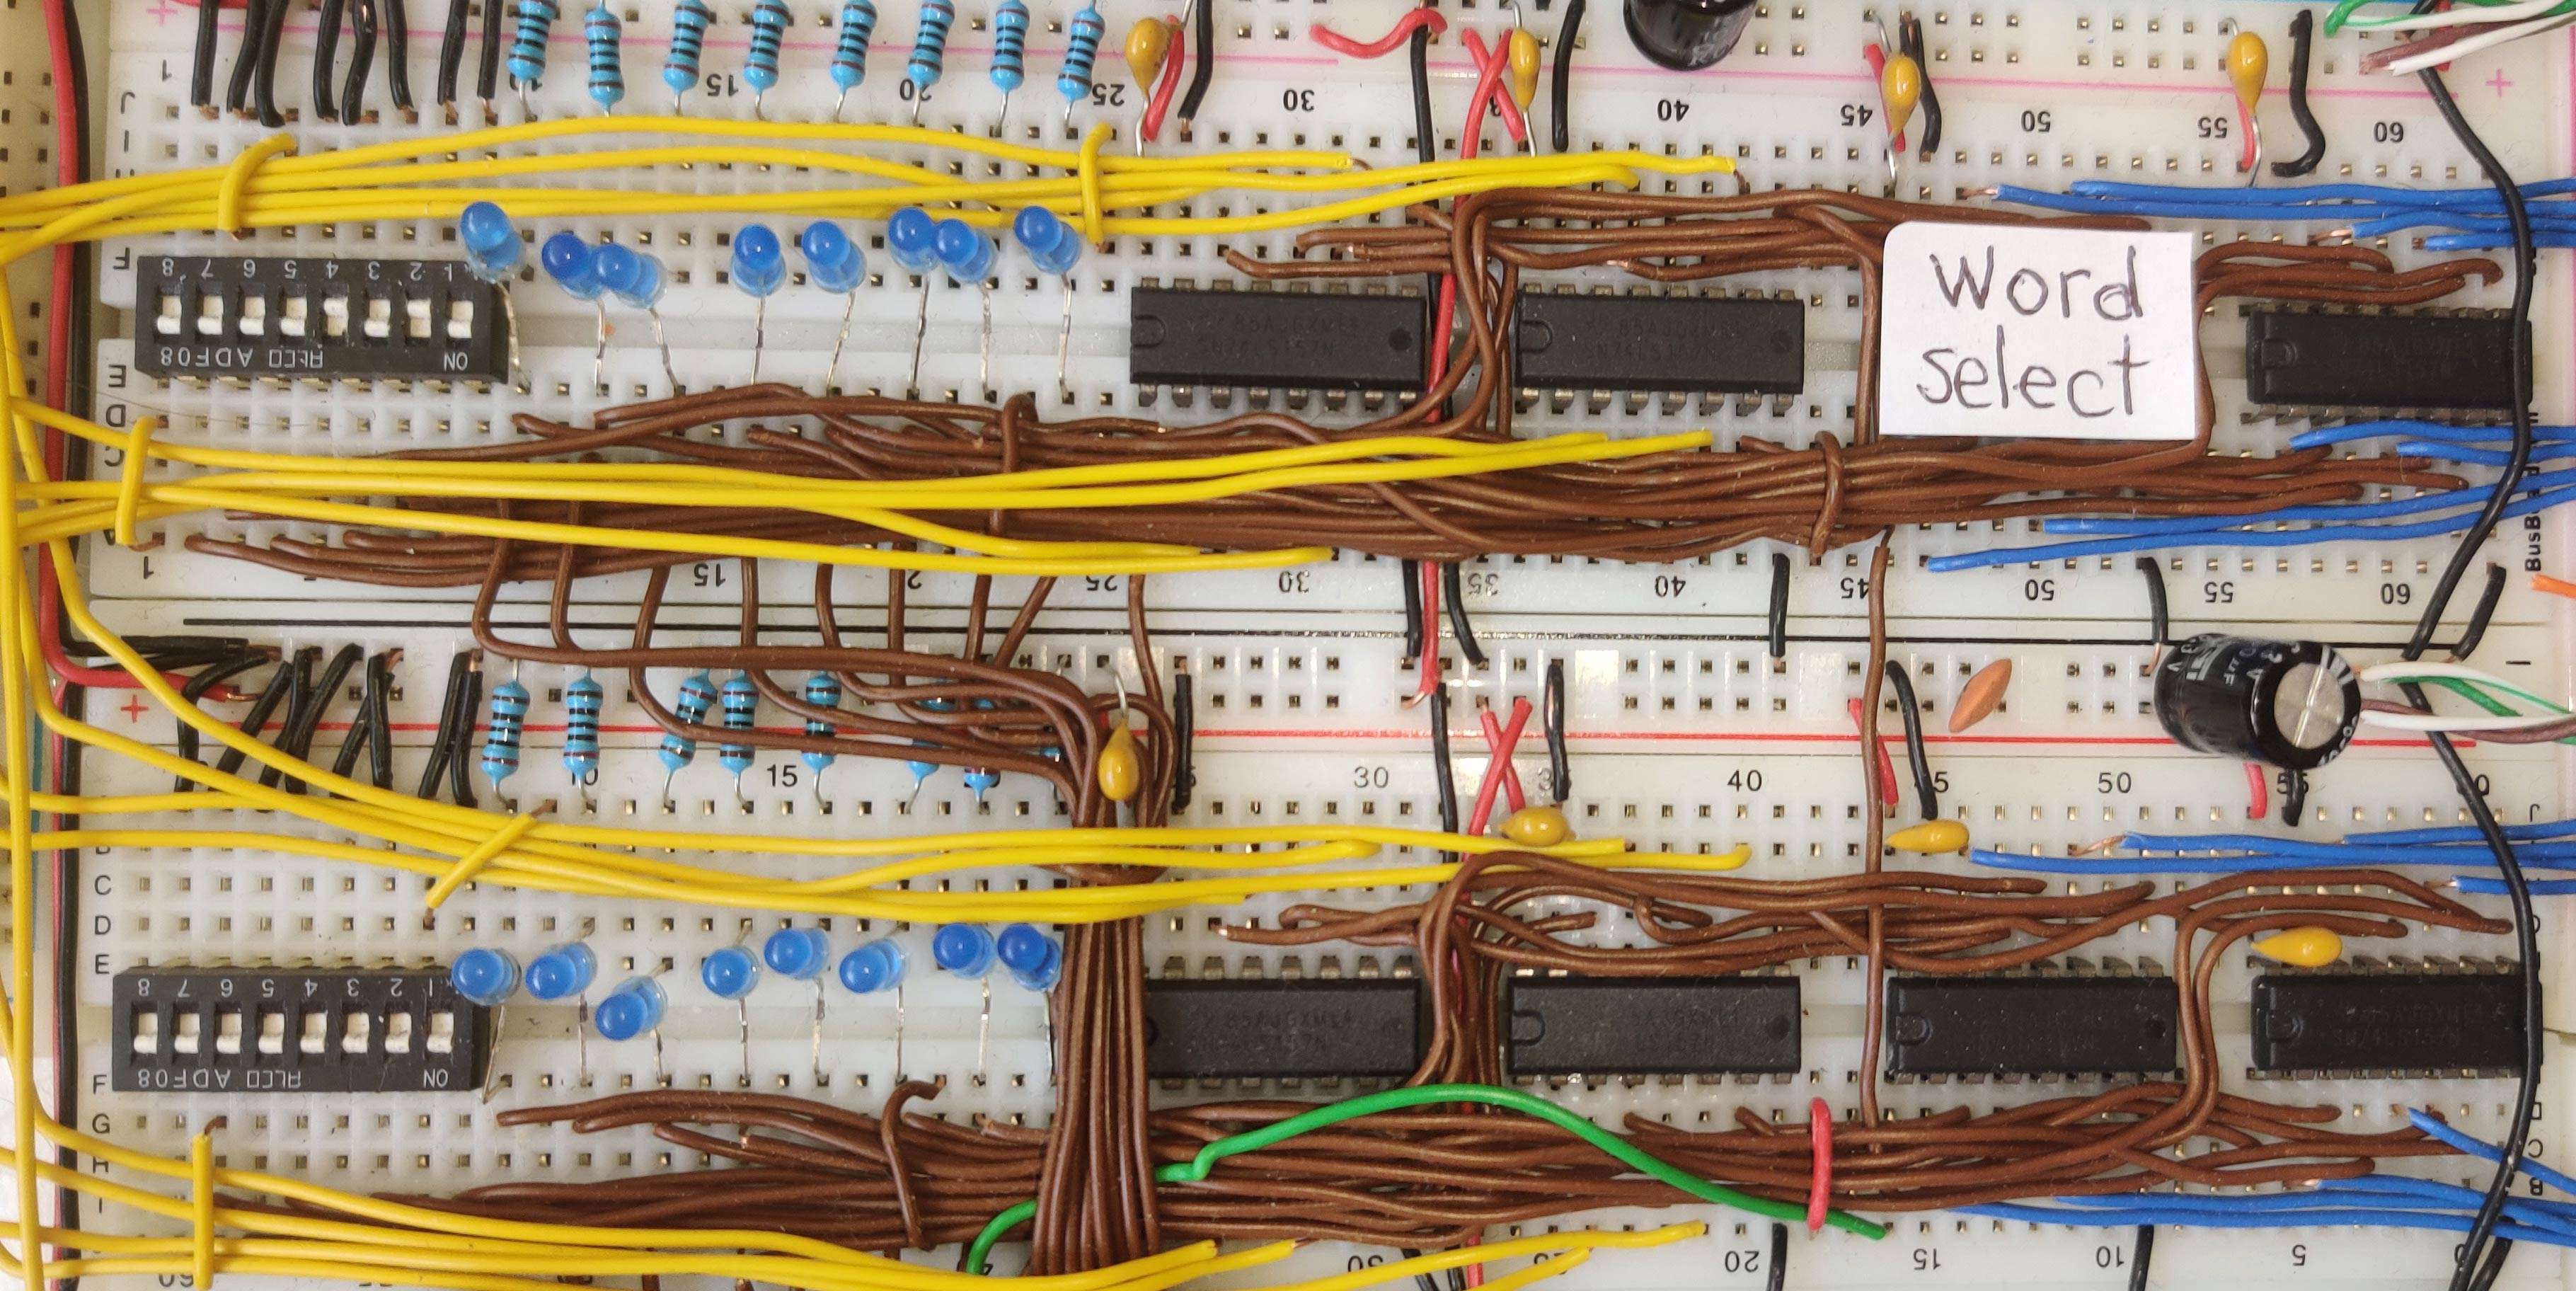
\includegraphics[scale=0.1]{comp/word-select}
    \caption{Word selector implementation}
    \label{word-select-i}
  \end{figure}

  \begin{figure}[h]
    \centering
    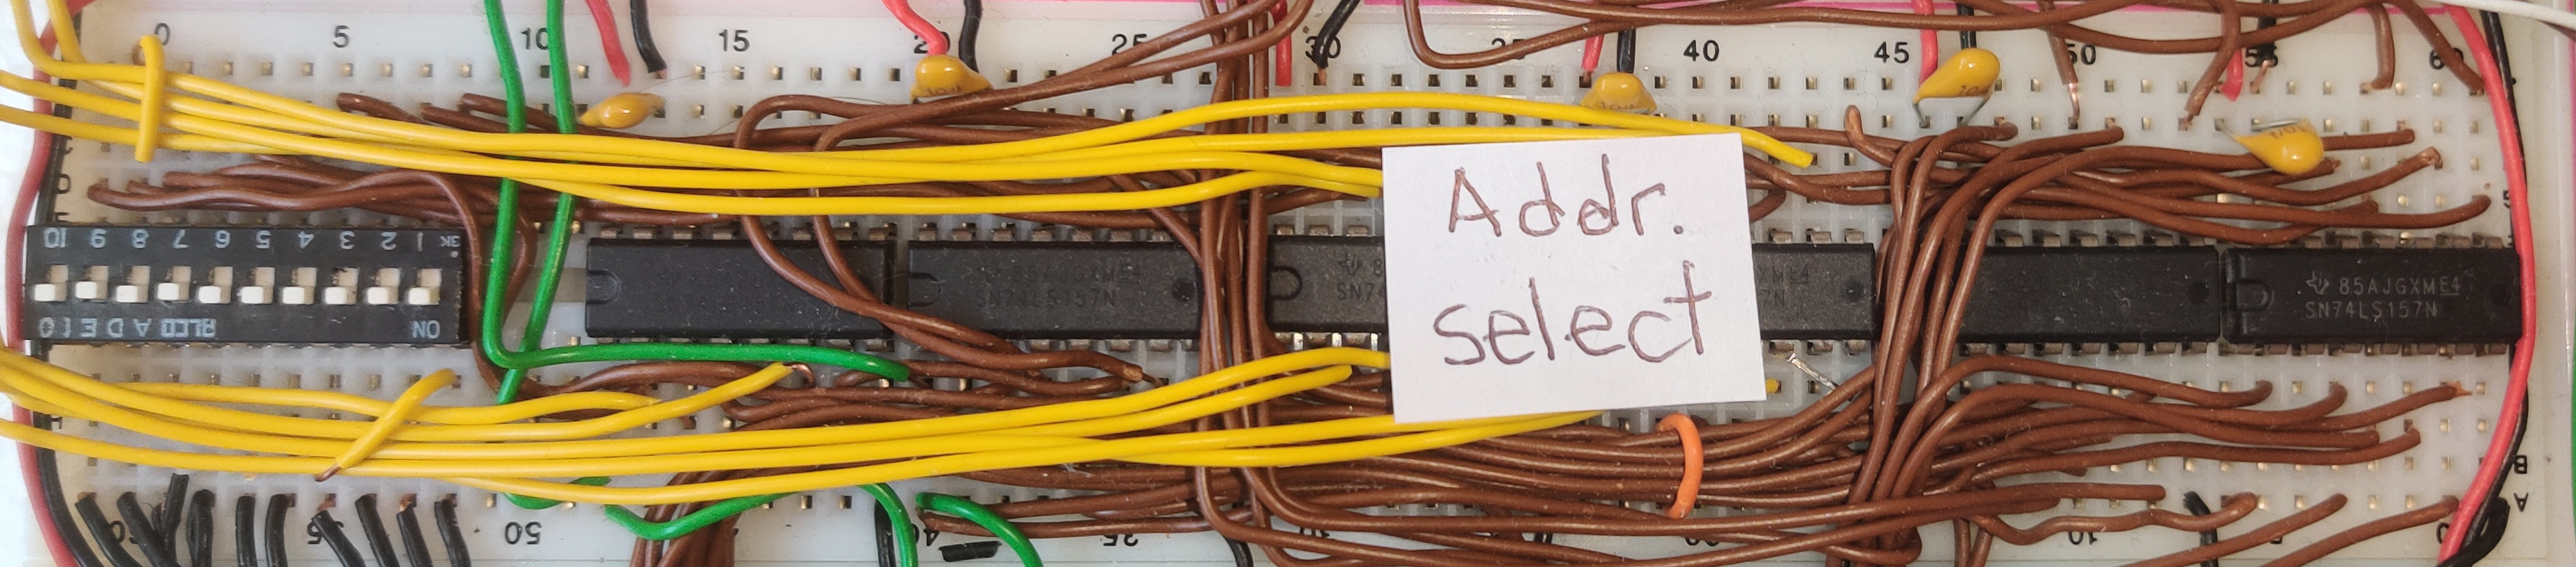
\includegraphics[scale=0.1]{comp/addr-select}
    \caption{Address selector implementation}
    \label{addr-select-i}
  \end{figure}

  \begin{figure}[h]
    \centering
    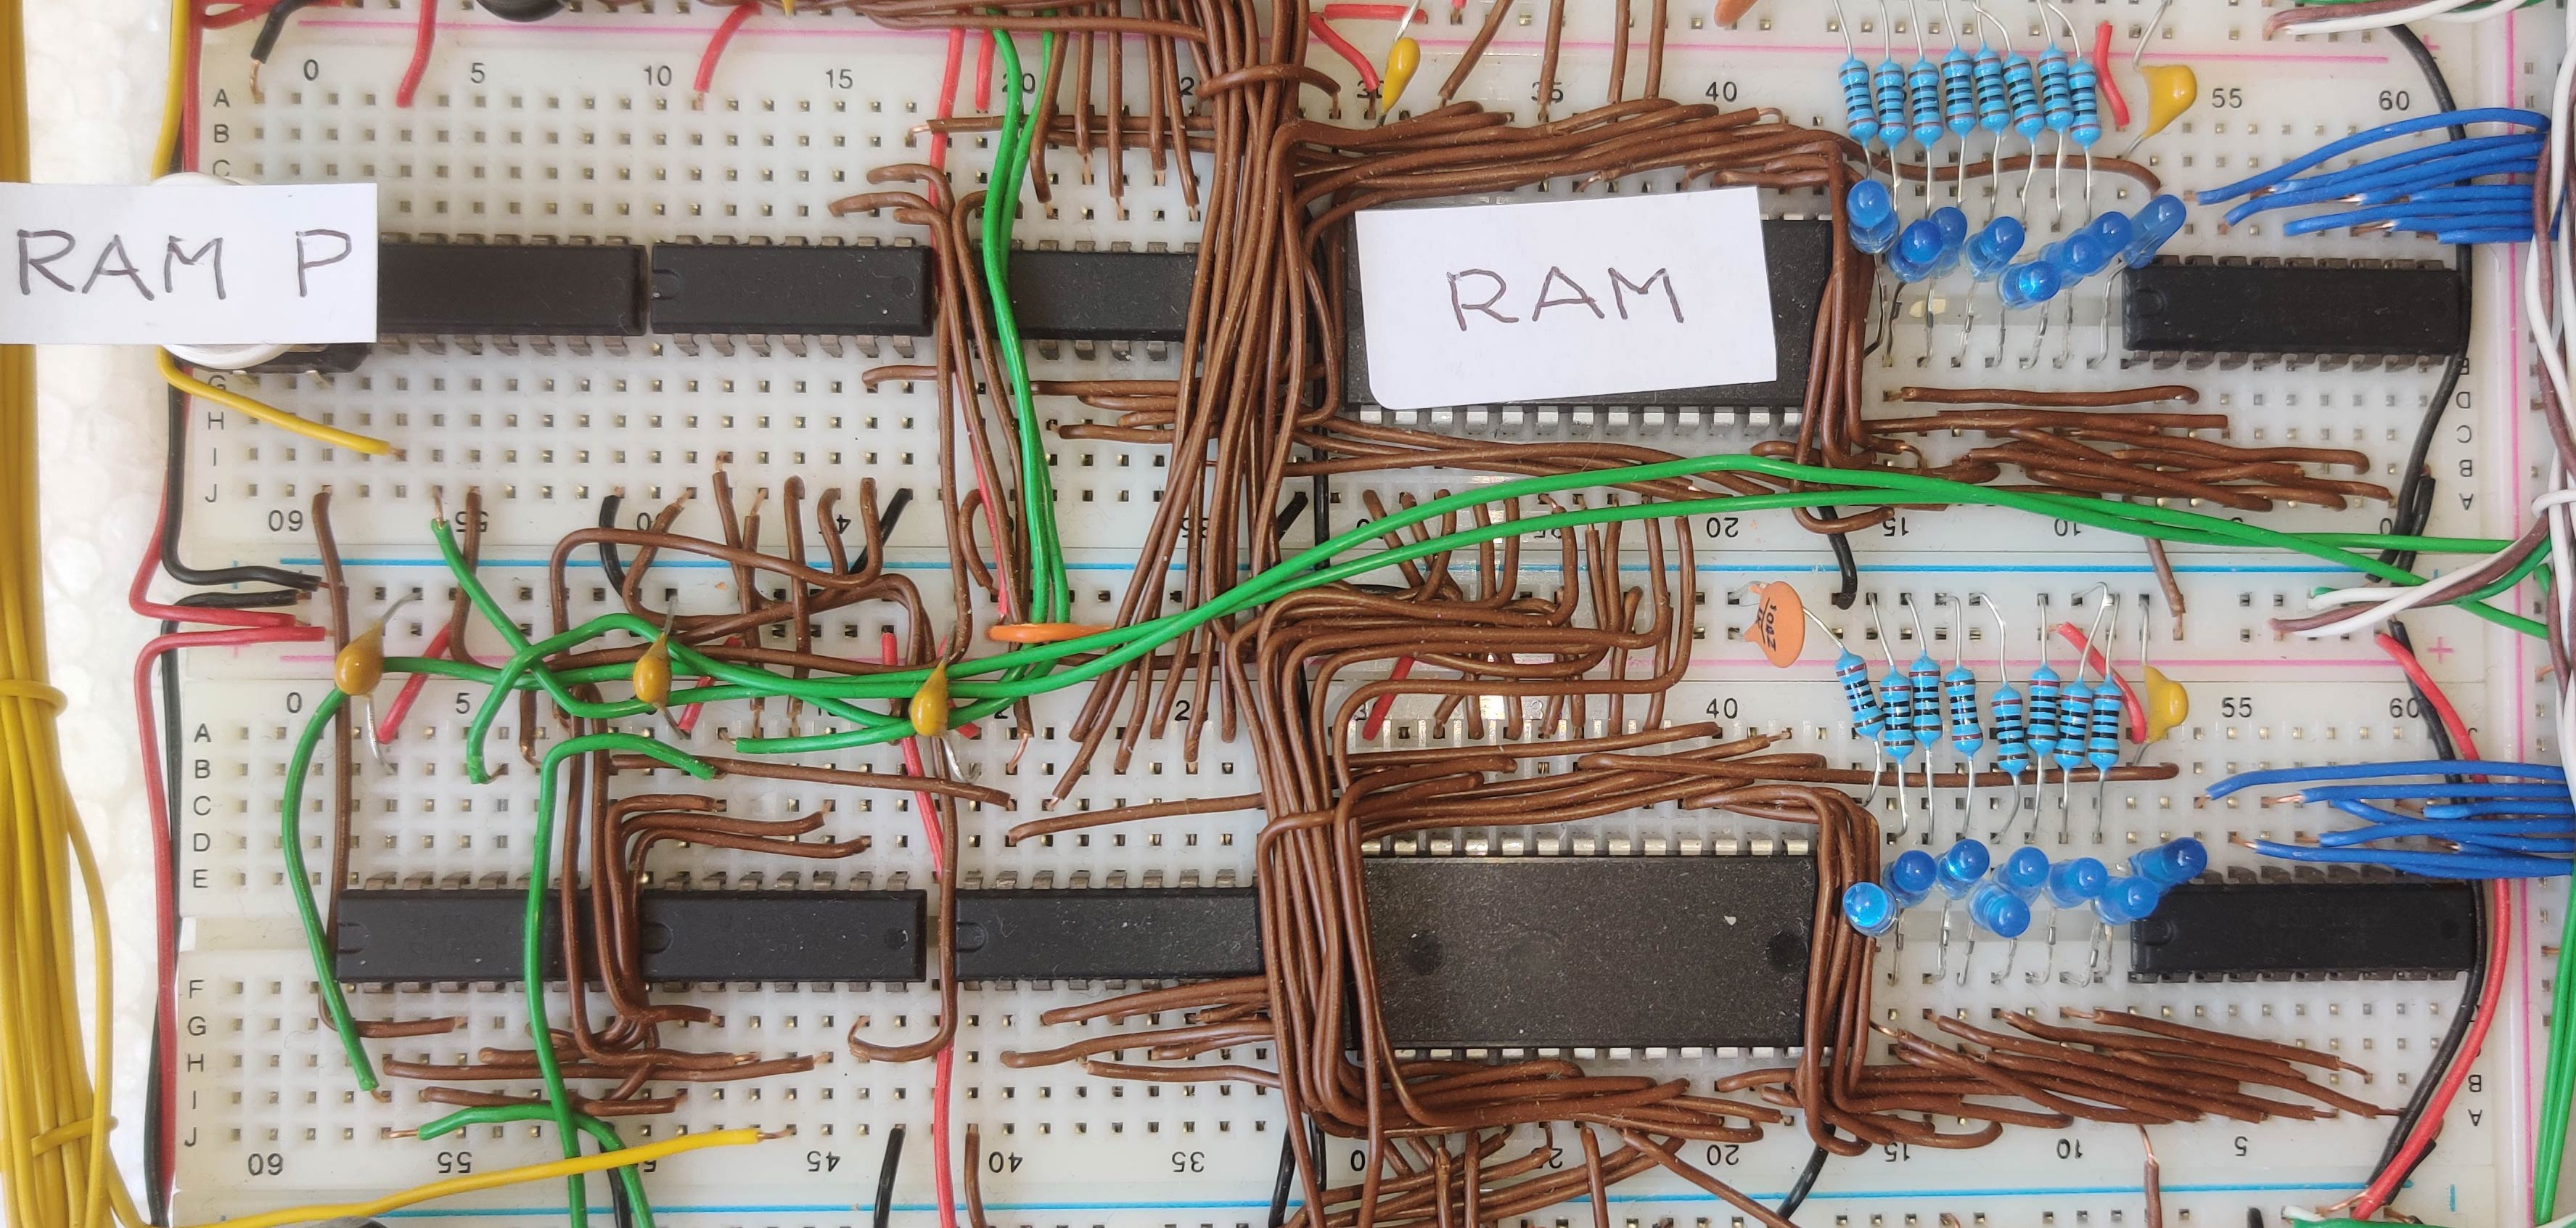
\includegraphics[scale=0.1]{comp/ram}
    \caption{Random Access Memory implementation}
    \label{ram-i}
  \end{figure}

  \begin{figure}[h]
    \centering
    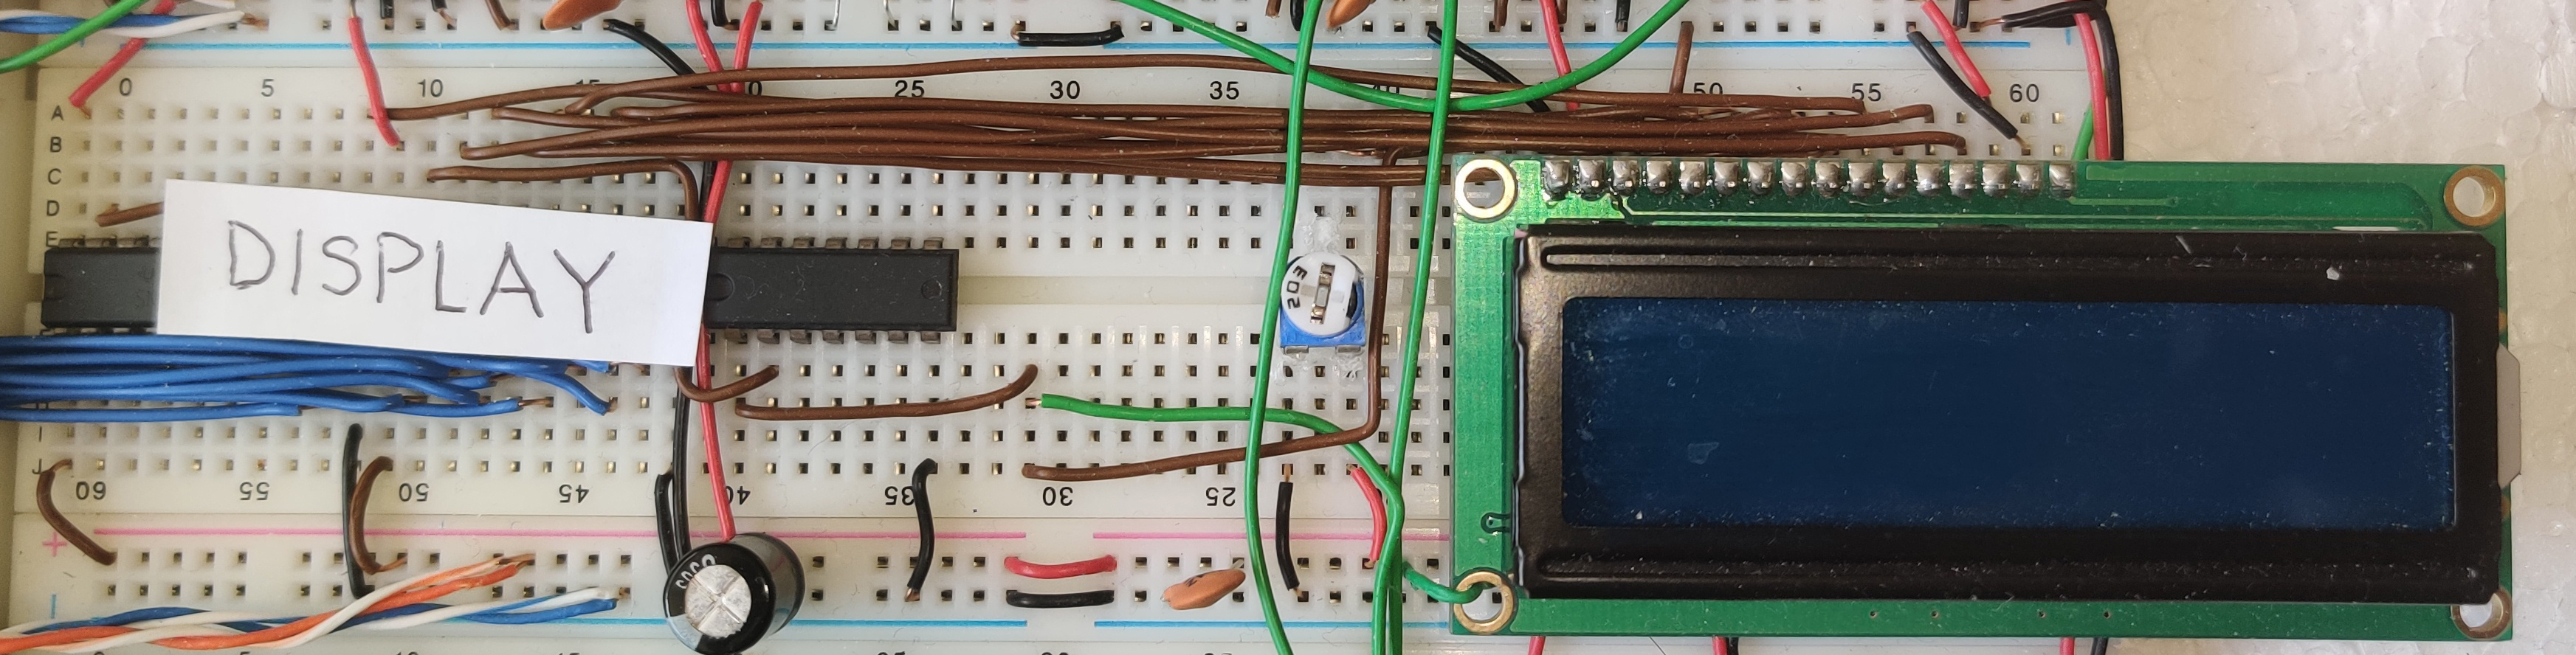
\includegraphics[scale=0.1]{comp/display}
    \caption{Display implementation}
    \label{display-i}
  \end{figure}

  \begin{figure}[h]
    \centering
    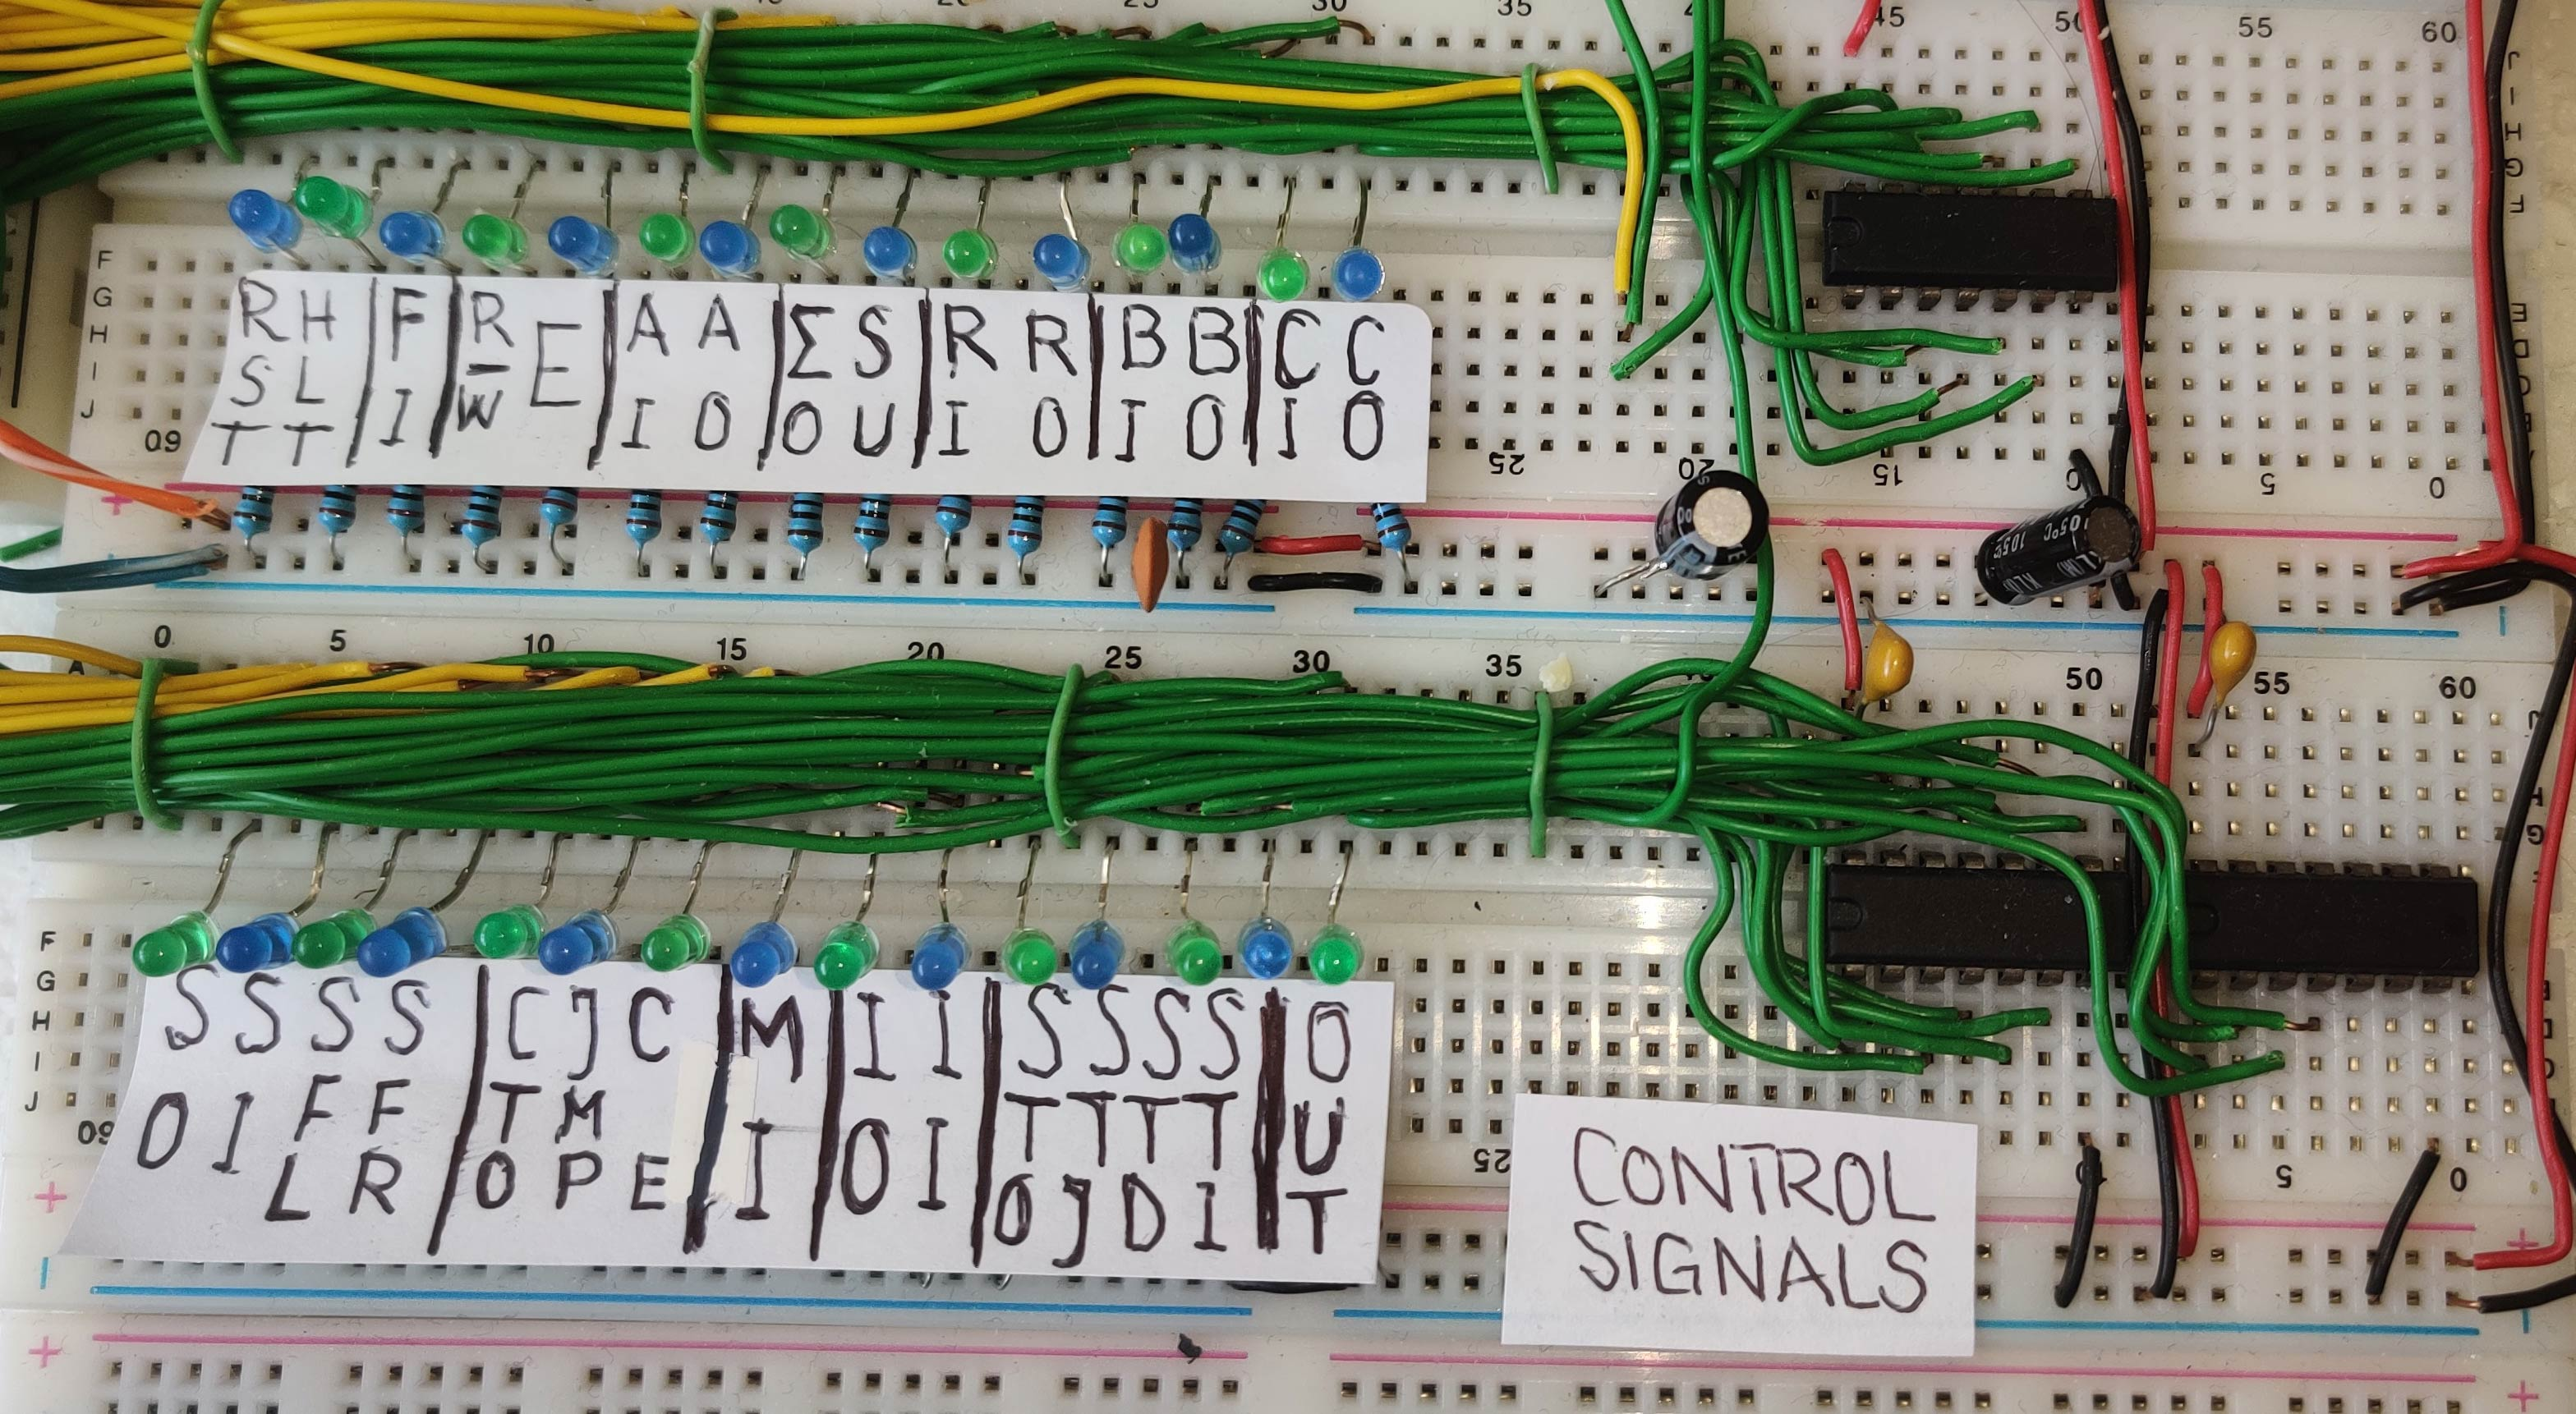
\includegraphics[scale=0.1]{comp/control-sigs}
    \caption{Implementation of the contol signals module}
    \label{control-sigs-i}
  \end{figure}

  \begin{figure}[h]
    \centering
    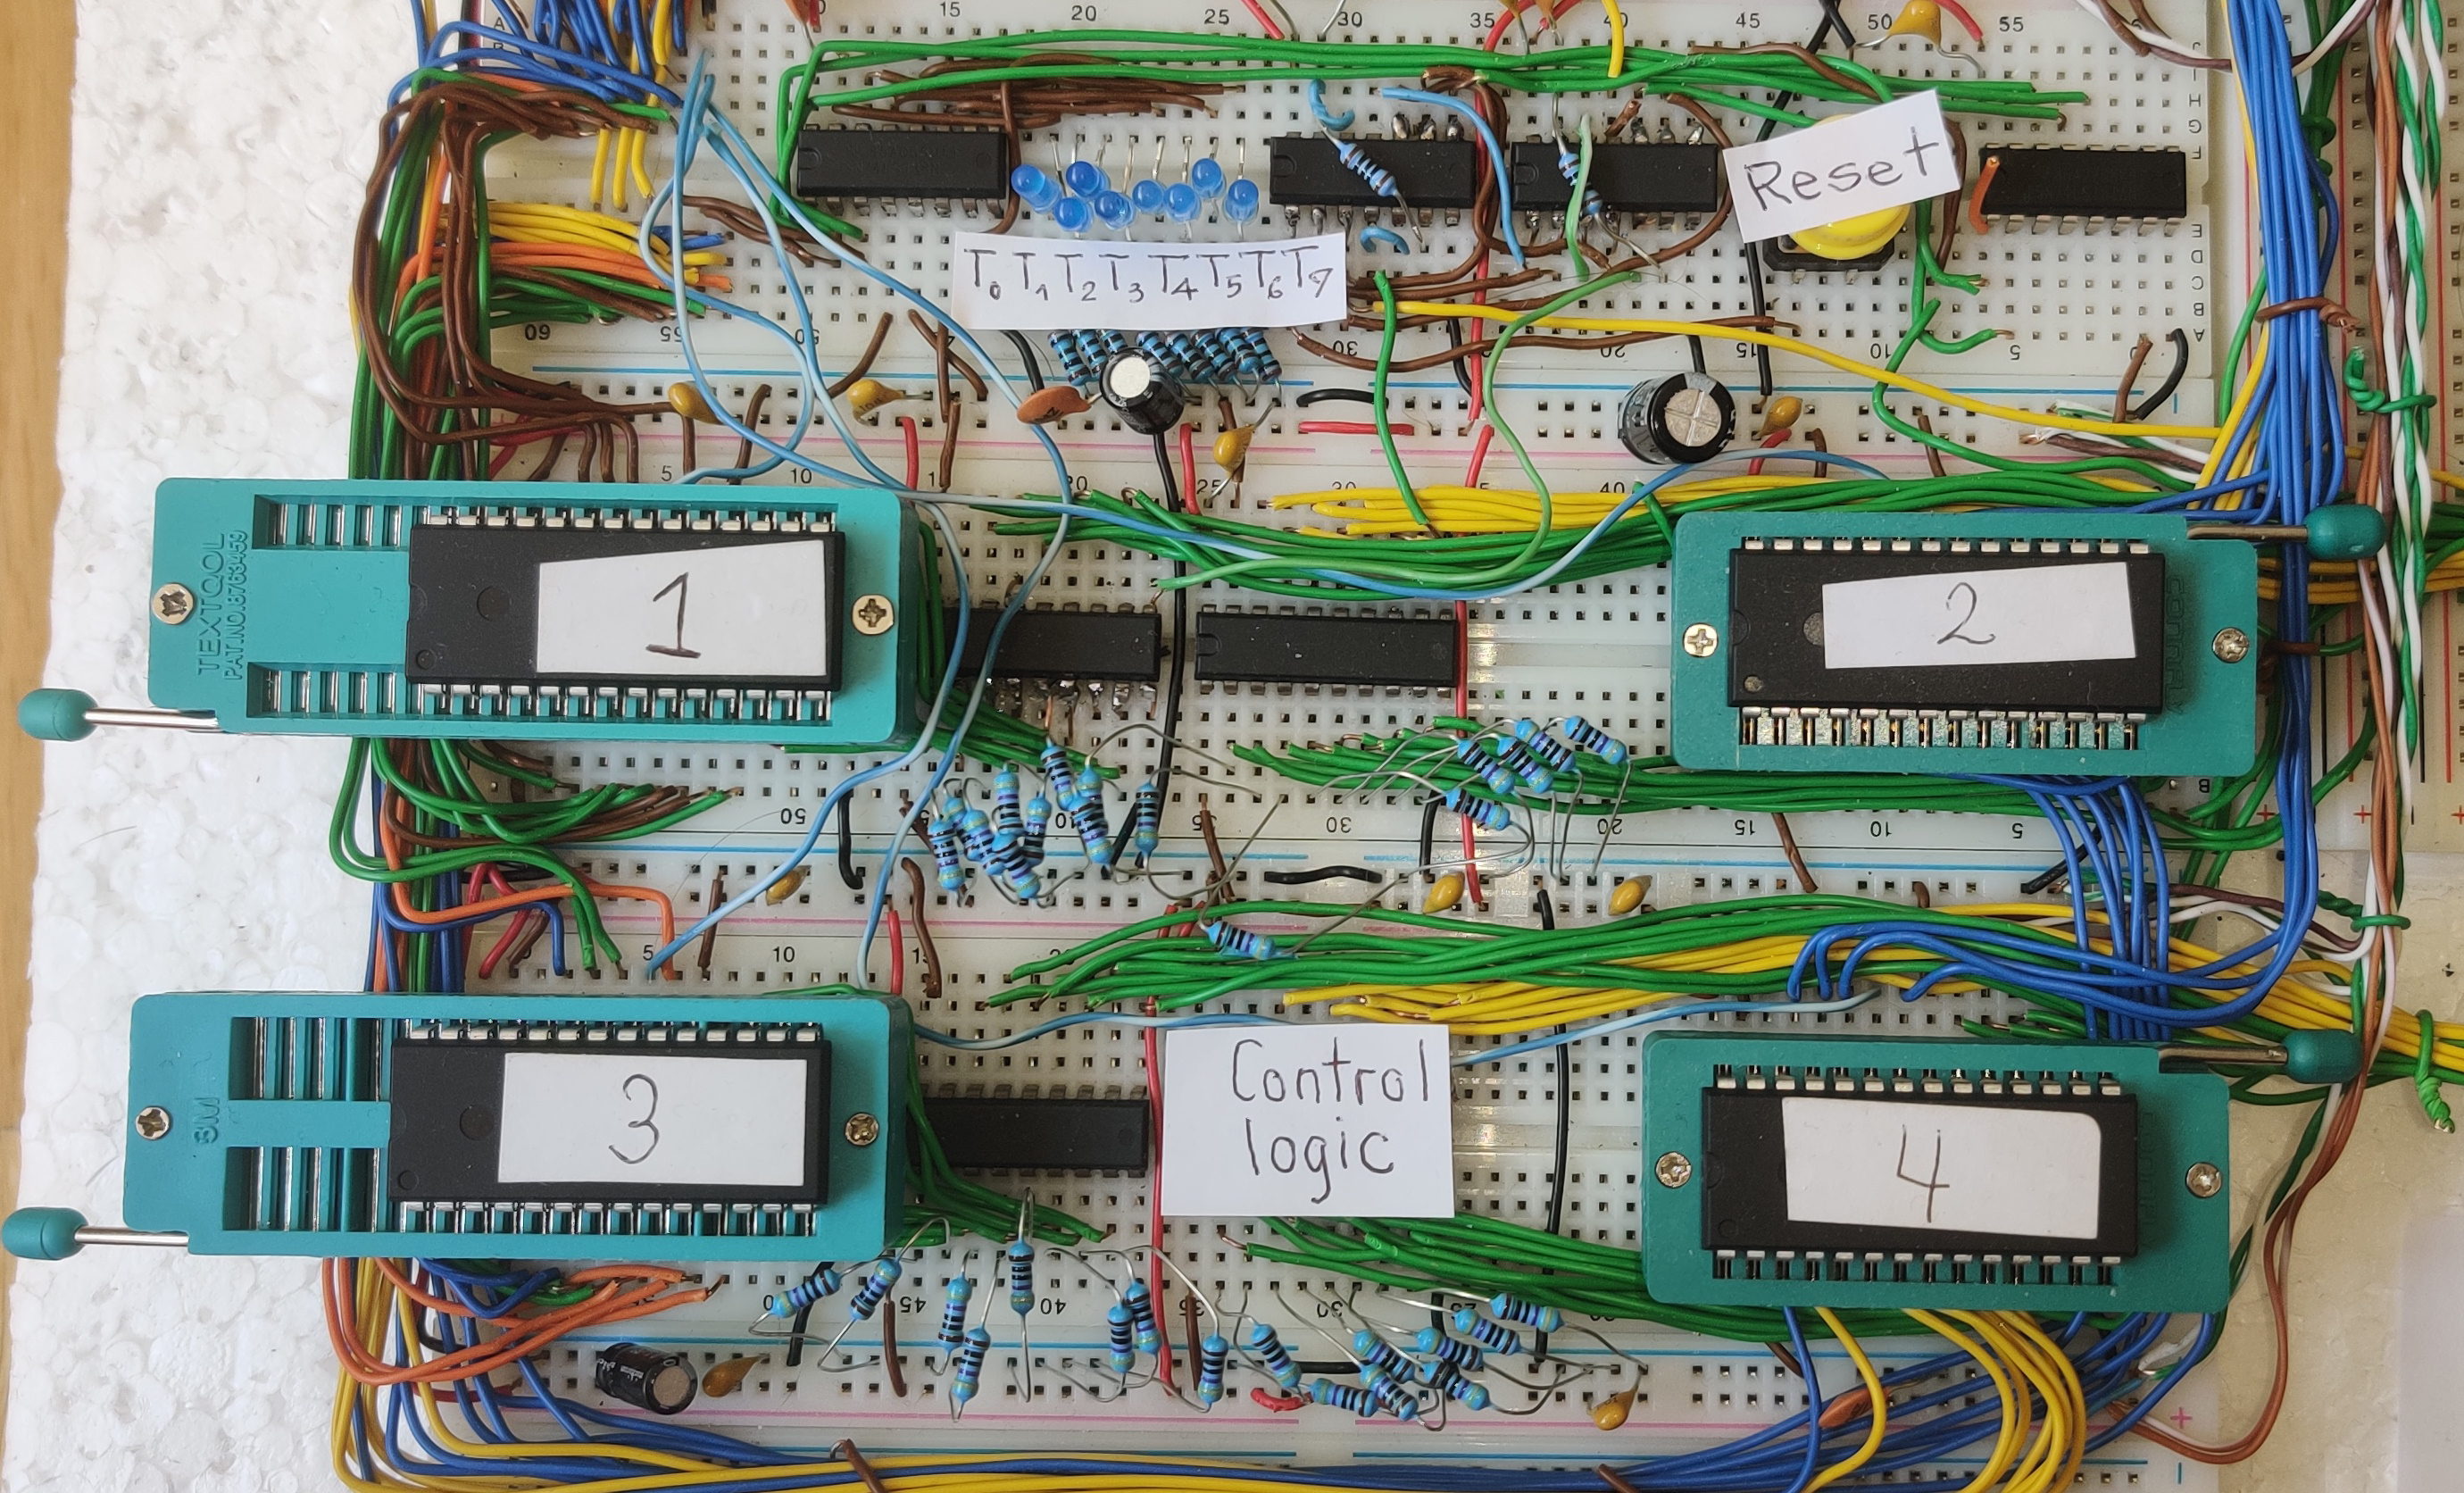
\includegraphics[scale=0.1]{comp/control-logic}
    \caption{Control Logic implementation}
    \label{control-logic-i}
  \end{figure}

  \begin{figure}[h]
    \centering
    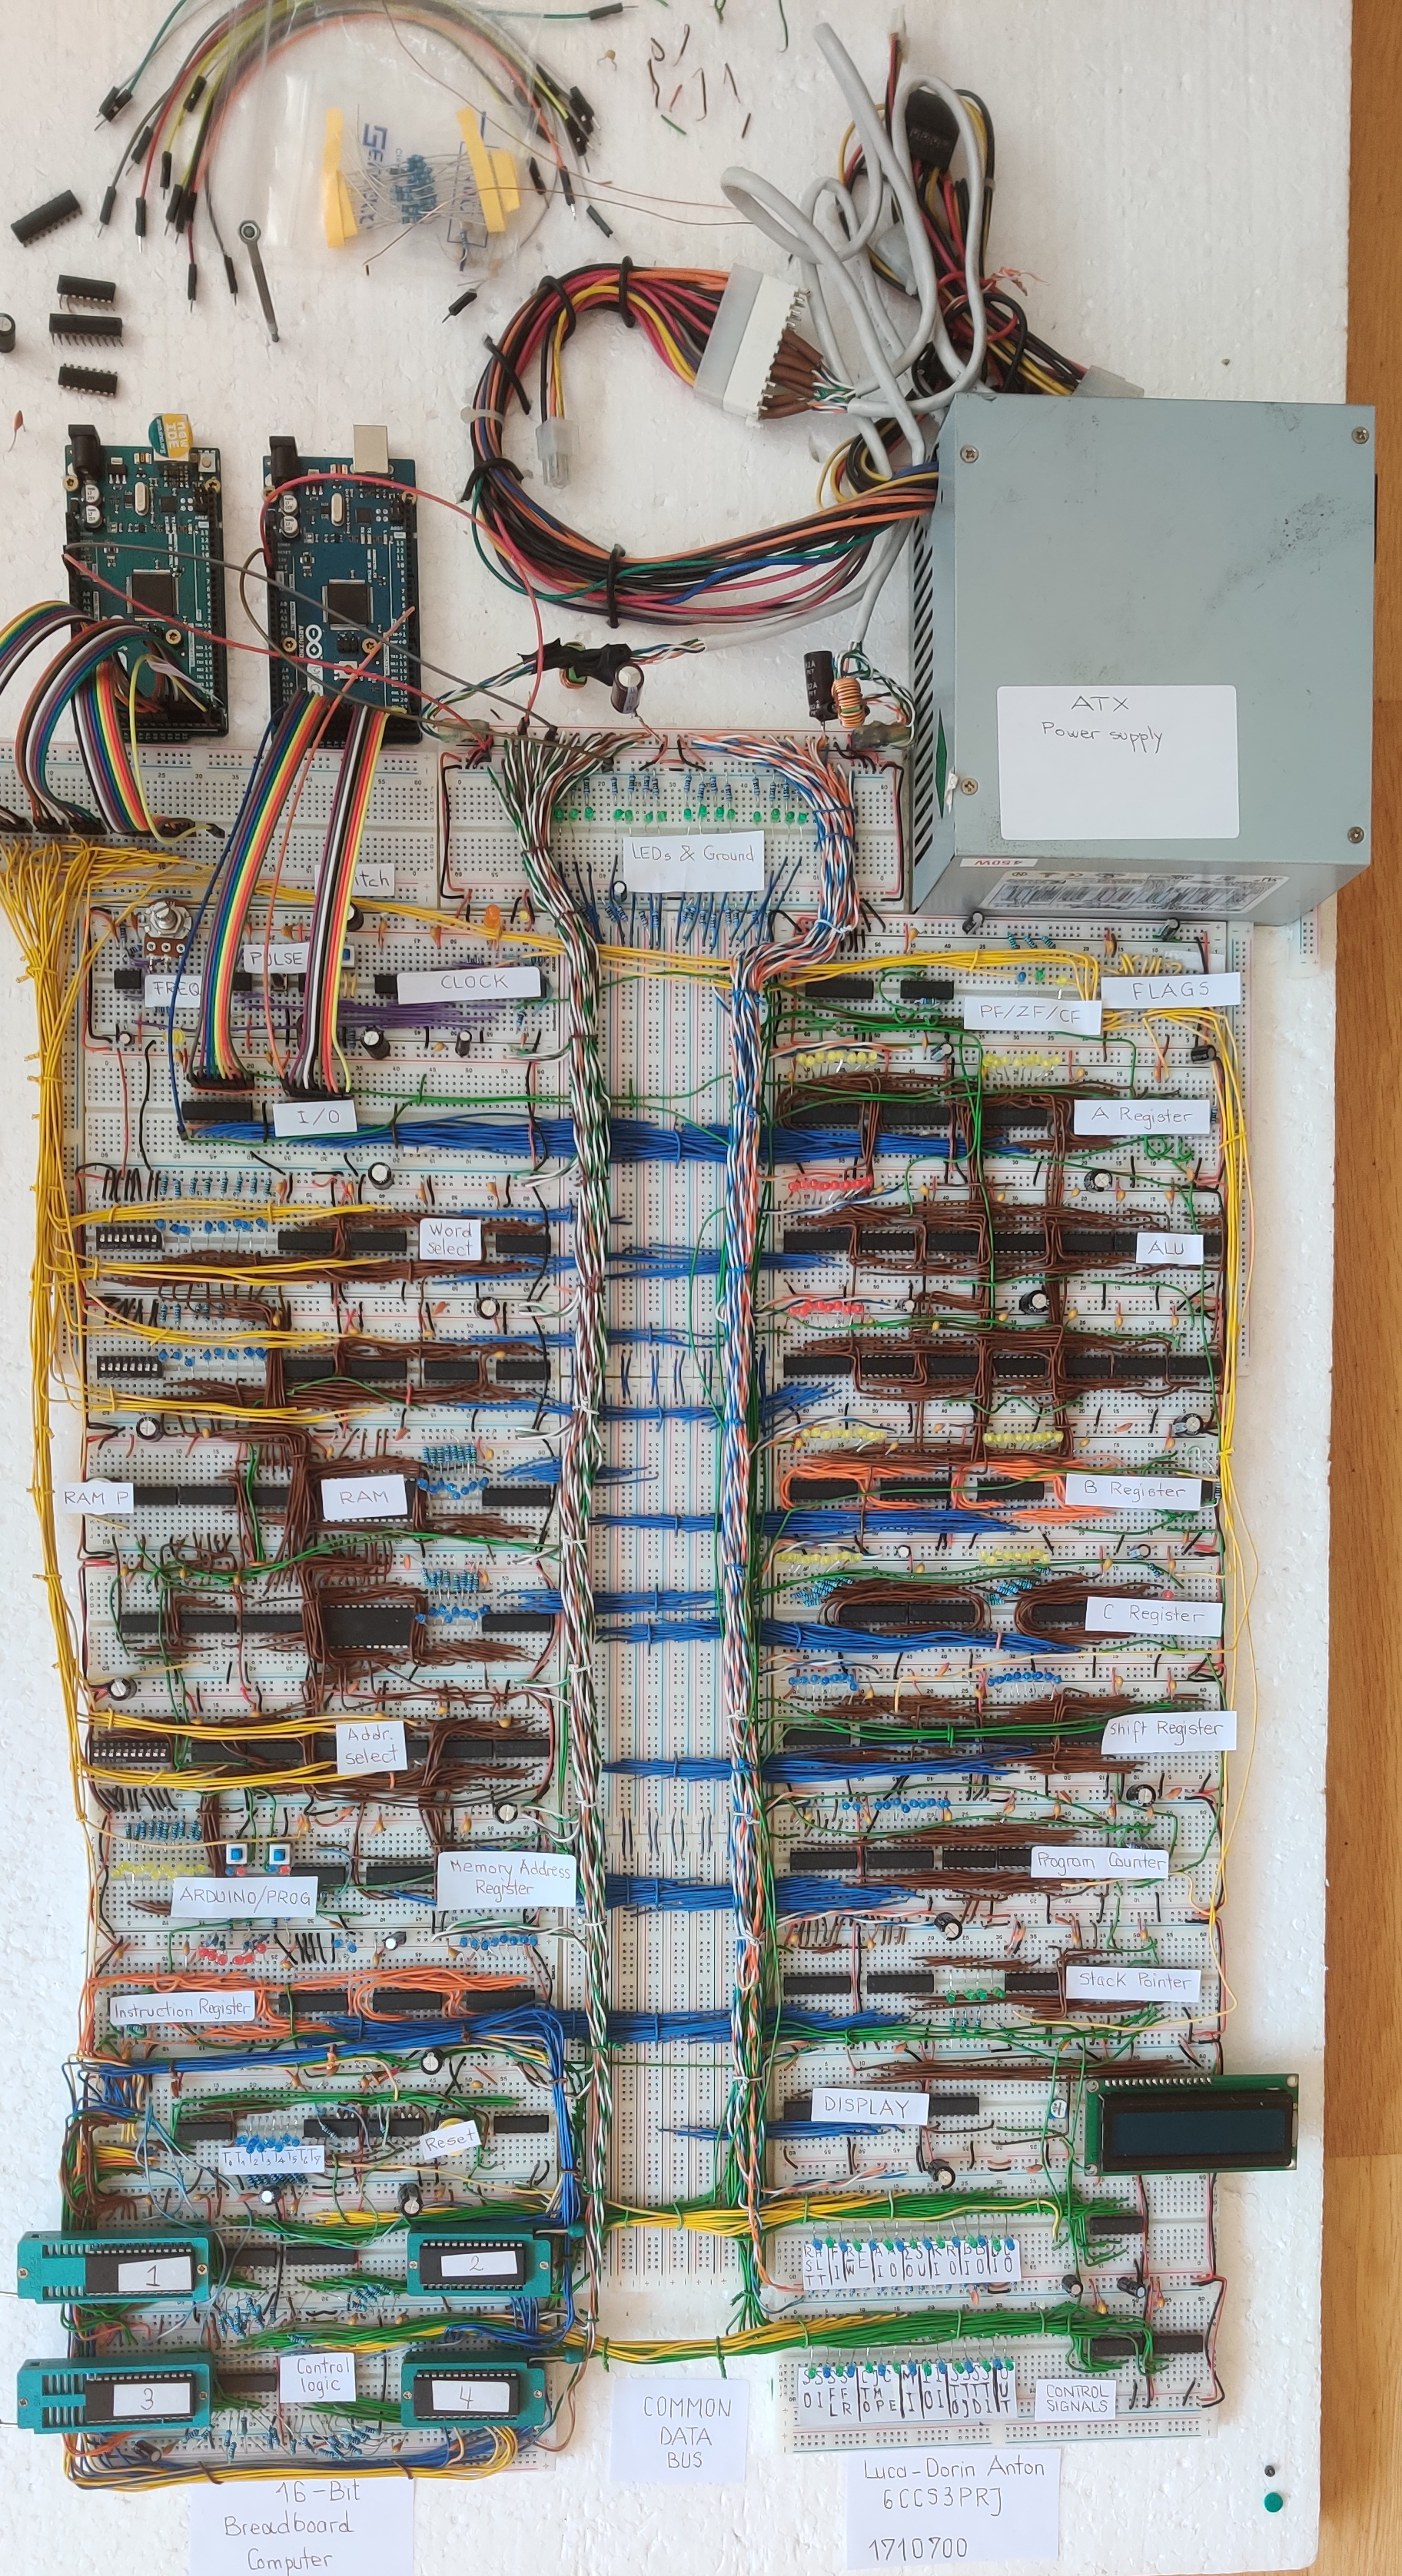
\includegraphics[scale=0.1]{comp/high-level}
    \caption{High level overview (with bus and LEDs visible)}
    \label{high-level-i}
  \end{figure}

\cleardoublepage
\cleardoublepage


After the first few modules and with enough power strips gathered, the first segment of the data
BUS was created. After that, all modules created so far were attached to the bus. From that point
on, after each module was built, it was attached to the bus. After a module was attached to the
bus, the direct connections to other modules which might exist were created. Initially, control
signals were connected with jumper wires, so that they could be manually turned on and off.
This was usefull for testing.


\section{Module Testing}
After the implementation of a module was completed, the next stage was to test it to ensure
it meets its specification. This was done by manually setting the control signals to either high
or low. To test using specific bus inputs, 16 jumper wires were connected to the bus, 1 to each
bud line, and then manually connected on a power strip to either high or low. This was used
to input bit patterns to a module to test that each bit was mapped correctly from the bus to the
module input and from the module output to the bus. Each module was tested this way.

\section{Implementation issues}
Implementation of most modules went through without significant issues. The main issue which
initially arrised was the power delivery. This prompted the switch from the simple phone charger
to the ATX power supply solution. Towards the end of the hardware implementation stage, a major
issue appeared.
\subsubsection{EEPROM issues}
After finalising the construction and connection of each module except for the control logic
module, all modules behaved as expected. Data could be read to and from the bus, the ALU would add
up number correctly, the program counter counted only when instructed, the display could receive
and dispplay instructions, RAM could be addressed correctly and manually programmed with success.
After the installation of the control logic module, issues started to arrise. Modules would
behave eratically, the counter on the clock module would count twice on every count cycle, it
would skip bits, ot sometimes not even count at all. Modules would read from the bus when they
weren't instructed to and sometimes short 'glitches' appeared on the LEDs module which monitored
the state of the bus. This issues would be removed if all the AT28C64B \cite{at28c64b} EEPROM
chips would be removed from their sockets. This prompted an investigation which ended up taking
over \textbf{one week of continuous work,} before the root of the problem was found. After many
different theories and patches without any effect, the issue ended up being not with the circuit,
but with the EEPROM chips themselves. According to the documentation, the chips have a 150 nano-
second time window after each address change in which they set up the output of the data contents
for the new address. During this very short time window, the output of the chips is
``undefined'' It seems that during this period, the undefined behaviour can equate to
significant voltage spikes. This voltage spikes, albeit short, are long enough to momentarily
change the state of the chips their are connected to (most \emph{74LS} are rated for clock speeds
of in the tens of MHz). This caused the unexpected behaviour. The sollution was a combination of
multiple patches:
\begin{itemize}
  \item \emph{Control Signals buffer chips: } Directly after the EEPROM chips, 4 \emph{74LS245}
  \cite{74ls245} buffer chips were installed. These chips have their advantage that their output
  is only logic 1 or 0, nothing in between, and that they amplify the signal going into them
  \item \emph{Pull-down Resistors: } 470 Ohm pull-down resistors were installed between the
  buffer chips and the EEPROM chips. This ensured that if the EEPROMs would have to drive to a
  relatively large voltge for a logic 1 input to be detected by the buffers
  \item \emph{RC filter networks: } On the most critical control signals \emph{RC networks}
  (Resistor - capacitor) networks were installed to filter out any potential voltage spikes.
  This circuits work by employing a very small capacitor which charges up very fast \ref{RCnet1}.
  This way, if a low frequency signal passes through the network, like the signals which are
  intended to be generated by the control logic module, it will quickly charge up the capacitor
  and then continue to propagate further on. This is intended. If a high frequency signal passes
  through the network, like for example the voltage spikes generated by the EEPROMs during address
  change, the signal won't have time to charge up the capacitor fully, and as such it won't
  propagate further thorugh the circuit. This filter circuit is then clamped between to
  gates (for example AND gates with inputs tied togheter or inverters) which are unused on the
  module where the singal is required, so as to ensure that the signal going in and out of the
  filter circuit is still digital. Then, the entire circuit is placed in series with the signal
  which it is supposed to filter. In practice in this case, 100 Ohm  resistors coupled with 10nF
  capacitors were used. These RC networks were placed on the \emph{CLK, RST, DONE, CE, AI, BI,
  II, MI} signals \ref{RCnet2}.
\end{itemize}

\begin{figure}[ht]
  \centering
  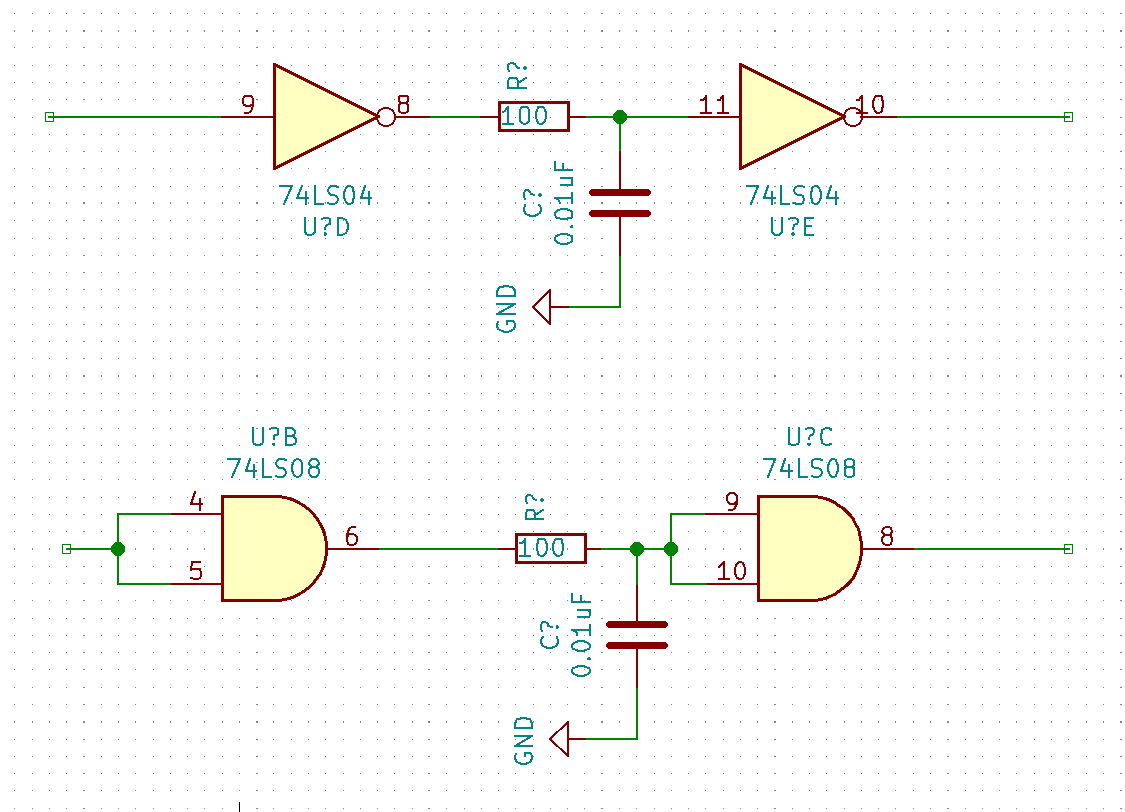
\includegraphics[scale=0.20]{RCnetwork}
  \caption{Example of AND-clamped and inverter-clamped RC networks in KiCad}
  \label{RCnet1}
\end{figure}

With this mitigation measures in place, the computer started behaving normally again.
